%% This template can be used to write a paper for
%% Computer Physics Communications using LaTeX.
%% For authors who want to write a computer program description,
%% an example Program Summary is included that only has to be
%% completed and which will give the correct layout in the
%% preprint and the journal.
%% The `elsarticle' style is used and more information on this style
%% can be found at 
%% http://www.elsevier.com/wps/find/authorsview.authors/elsarticle.
%%

%% Use the option review to obtain double line spacing
% \documentclass[preprint,12pt]{elsarticle}

%% Use the options 1p,twocolumn; 3p; 3p,twocolumn; 5p; or 5p,twocolumn
%% for a journal layout:
% \documentclass[final,1p,times]{elsarticle}
% \documentclass[final,1p,times,twocolumn]{elsarticle}
\documentclass[final,3p,times]{elsarticle}
% \documentclass[final,3p,times,twocolumn]{elsarticle}
% \documentclass[final,5p,times]{elsarticle}
% \documentclass[final,5p,times,twocolumn]{elsarticle}

\usepackage{subcaption}
\usepackage[newfloat]{minted}
\usepackage{hyperref}
\usepackage{tcolorbox}
\usepackage{etoolbox}
\BeforeBeginEnvironment{minted}{\begin{center}\begin{tcolorbox}[width=0.9\textwidth]}
\AfterEndEnvironment{minted}{\end{tcolorbox}\end{center}}
% \usemintedstyle[python]{vs}
\usepackage{caption}
\usepackage{xspace}
\usepackage[toc,page]{appendix}

\newcommand{\inline}[1]{\mintinline{python}{#1}\xspace}
\newcommand{\SuperScreen}{\inline{SuperScreen}}

\newenvironment{code}{\captionsetup{type=listing}}{\hfill}
\SetupFloatingEnvironment{listing}{name=Code Block}
\BeforeBeginEnvironment{code}{\vspace{10pt}\begin{minipage}{\textwidth}}
\AfterEndEnvironment{code}{\end{minipage}}
\captionsetup[listing]{skip=0pt}

%% if you use PostScript figures in your article
%% use the graphics package for simple commands
%% \usepackage{graphics}
%% or use the graphicx package for more complicated commands
%% \usepackage{graphicx}
%% or use the epsfig package if you prefer to use the old commands
%% \usepackage{epsfig}

%% The amssymb package provides various useful mathematical symbols
\usepackage{amsmath, amssymb, bm}
%% The amsthm package provides extended theorem environments
%% \usepackage{amsthm}

%% The lineno packages adds line numbers. Start line numbering with
%% \begin{linenumbers}, end it with \end{linenumbers}. Or switch it on
%% for the whole article with \linenumbers after \end{frontmatter}.
%% \usepackage{lineno}

%% natbib.sty is loaded by default. However, natbib options can be
%% provided with \biboptions{...} command. Following options are
%% valid:

%%   round  -  round parentheses are used (default)
%%   square -  square brackets are used   [option]
%%   curly  -  curly braces are used      {option}
%%   angle  -  angle brackets are used    <option>
%%   semicolon  -  multiple citations separated by semi-colon
%%   colon  - same as semicolon, an earlier confusion
%%   comma  -  separated by comma
%%   numbers-  selects numerical citations
%%   super  -  numerical citations as superscripts
%%   sort   -  sorts multiple citations according to order in ref. list
%%   sort&compress   -  like sort, but also compresses numerical citations
%%   compress - compresses without sorting
%%
%% \biboptions{comma,round}

% \biboptions{}

%% This list environment is used for the references in the
%% Program Summary
%%
\newcounter{bla}
\newenvironment{refnummer}{%
\list{[\arabic{bla}]}%
{\usecounter{bla}%
 \setlength{\itemindent}{0pt}%
 \setlength{\topsep}{0pt}%
 \setlength{\itemsep}{0pt}%
 \setlength{\labelsep}{2pt}%
 \setlength{\listparindent}{0pt}%
 \settowidth{\labelwidth}{[9]}%
 \setlength{\leftmargin}{\labelwidth}%
 \addtolength{\leftmargin}{\labelsep}%
 \setlength{\rightmargin}{0pt}}}
 {\endlist}

\journal{Computer Physics Communications}

\begin{document}

\begin{frontmatter}

%% Title, authors and addresses

%% use the tnoteref command within \title for footnotes;
%% use the tnotetext command for the associated footnote;
%% use the fnref command within \author or \address for footnotes;
%% use the fntext command for the associated footnote;
%% use the corref command within \author for corresponding author footnotes;
%% use the cortext command for the associated footnote;
%% use the ead command for the email address,
%% and the form \ead[url] for the home page:
%%
%% \title{Title\tnoteref{label1}}
%% \tnotetext[label1]{}
%% \author{Name\corref{cor1}\fnref{label2}}
%% \ead{email address}
%% \ead[url]{home page}
%% \fntext[label2]{}
%% \cortext[cor1]{}
%% \address{Address\fnref{label3}}
%% \fntext[label3]{}

\title{\texttt{SuperScreen}: An open-source package for simulating the magnetic response of two-dimensional superconducting devices}

%% use optional labels to link authors explicitly to addresses:
%% \author[label1,label2]{<author name>}
%% \address[label1]{<address>}
%% \address[label2]{<address>}

\author[PHYS,SIMES]{Logan Bishop-Van Horn}
\author[AP,SIMES,GLAM]{Kathryn A. Moler\corref{author}}

\cortext[author]{Corresponding author.\\\textit{E-mail address:} kmoler@stanford.edu}

\address[PHYS]{Department of Physics, Stanford University, Stanford, California 94305, USA}
\address[AP]{Department of Applied Physics, Stanford University, Stanford, California 94305, USA}
\address[SIMES]{Stanford Institute for Materials and Energy Sciences, SLAC National Accelerator Laboratory, 2575 Sand Hill Road, Menlo Park, California 94025, USA}
\address[GLAM]{Geballe Laboratory for Advanced Materials, Stanford University, Stanford, California 94305, USA}

\begin{abstract}
Quantitative understanding of the spatial distribution of magnetic fields and screening currents in two-dimensional (2D) superconductors and mesoscopic thin film superconducting devices is critical to interpreting the results of magnetic measurements of such systems. Here, we introduce \SuperScreen, an open-source Python package for simulating the magnetic response of 2D superconductors to applied time-independent magnetic fields. Given an applied magnetic field, \SuperScreen solves for the Meissner currents and magnetic fields in and around structures composed of one or more superconducting thin films of arbitrary geometry with spatially inhomogeneous magnetic penetration depth using an efficient matrix inversion method~\cite{Brandt2004-ew, Brandt2005-wj}. \SuperScreen can be used to model screening effects and calculate self- and mutual-inductance in superconducting circuits, and simulate the magnetic response of inhomogeneous 2D superconductors.
\end{abstract}

\begin{keyword}
%% keywords here, in the form: keyword \sep keyword
superconductivity\sep Meissner screening\sep thin film\sep London equations \sep inductance

\end{keyword}

\end{frontmatter}

%%
%% Start line numbering here if you want
%%
% \linenumbers

% All CPiP articles must contain the following
% PROGRAM SUMMARY.
\noindent
{\bf PROGRAM SUMMARY}

\begin{small}
\noindent
{\em SuperScreen}\\
{\em CPC Library link to program files:} (to be added by Technical Editor) \\
{\em Developer's repository link:} \href{http://www.github.com/loganbvh/superscreen}{www.github.com/loganbvh/superscreen}\\
{\em Code Ocean capsule:} (to be added by Technical Editor)\\
{\em Licensing provisions:} MIT\\
{\em Programming language: Python}\\
% {\em Supplementary material:}\\
  % Fill in if necessary, otherwise leave out.
% {\em Journal reference of previous version:}*\\
  %Only required for a New Version summary, otherwise leave out.
% {\em Does the new version supersede the previous version?:}*\\
  %Only required for a New Version summary, otherwise leave out.
% {\em Reasons for the new version:*}\\
  %Only required for a New Version summary, otherwise leave out.
% {\em Summary of revisions:}*\\
  %Only required for a New Version summary, otherwise leave out.
{\em Nature of problem:} \SuperScreen solves for Meissner screening currents in structures composed of 2D or thin film superconductors in the presence of an applied magnetic field, pinned vortices, and trapped flux.\\
  %Describe the nature of the problem here. \\
{\em Solution method:} This package solves the 2D London equation for superconducting thin films using a matrix inversion method~\cite{Brandt2004-ew,Brandt2005-wj}.\\
  %Describe the method solution here.
% {\em Additional comments including restrictions and unusual features (approx. 50-250 words):}\\
  %Provide any additional comments here.
   \\

% \begin{thebibliography}{0}
% \bibitem{1}Reference 1         % This list should only contain those items referenced in the                 
% \bibitem{2}Reference 2         % Program Summary section.   
% \bibitem{3}Reference 3         % Type references in text as [1], [2], etc.
%                               % This list is different from the bibliography at the end of 
%                               % the Long Write-Up.
% \end{thebibliography}
\end{small}


%% main text
\section{Introduction}
\label{section:introduction}

\SuperScreen is a Python package developed to simulate the static magnetic response of structures composed of one or more layers containing superconducting thin films. \SuperScreen solves the coupled Maxwell's and London's equations in and around superconducting films with spatially-varying penetration depth in the presence of inhomogeneous applied magnetic fields, pinned vortices, and trapped flux using a matrix inversion method introduced by Brandt and Clem~\cite{Brandt2004-ew,Brandt2005-wj} and subsequently used by Kirtley, \emph{et al.} to model the magnetic response of scanning superconducting quantum interference device (SQUID) sensors.~\cite{Kirtley2016-zz, Kirtley2016-gt}

There have been many previous numerical studies of magnetic screening and inductance extraction in thin film and two-dimensional (2D) superconducting devices~\cite{Jaycox1981-zl, Ketchen1982-at, Ketchen2012-mb, Hildebrandt1995-uw, Khapaev1997-kw, Khapaev2001-xq, Khapaev2001-pw, Babaei_Brojeny2003-la, Brandt2004-ew, Brandt2005-wj, Clem2005-ye, Muller2021-ci, Jackman2016-mf}. However, few software tools for this task exist and those that are available are closed-source, are written in low-level compiled languages like C, and/or require the use of specialized file formats or separate computer aided design (CAD) software for defining device geometries and model configurations.\footnote{A brief summary of existing tools can be found in \ref{appendix:other-tools}, and a more thorough overview in Ref.~\cite{Gaj1999-ls}.} Most of these tools are intended for use in the design of superconducting integrated circuits for rapid single flux quantum (RSFQ) logic and are primarily used for inductance extraction~\cite{Gaj1999-ls}. In contrast, \SuperScreen is an open-source, user-friendly, portable research tool designed to lower the barrier to entry to quantitative modeling of 2D superconductors, and to help interpret and inform measurements of superconducting thin films and devices.

This introduction to \SuperScreen is organized as follows: In Section~\ref{section:model}, we outline the model and its assumptions and in Section~\ref{section:implementation}, we describe its numerical implementation. In Section~\ref{section:overview}, we provide an overview of the structure of the \SuperScreen package and discuss some important development details. In Section~\ref{section:examples}, we demonstrate how to perform several types of simulations using \SuperScreen and compare the results to previous numerical/analytical solutions and experimental results. Finally, in Section~\ref{section:conlusion}, we conclude by discussing applications, limitations, and possible extensions of the package.

\section{The Model}
\label{section:model}

The goal of \SuperScreen is to model the magnetic response of a thin superconducting film, or a structure composed of multiple superconducting films (which may or may not lie in the same plane), to an applied inhomogeneous out-of-plane magnetic field
$H_{z,\,\mathrm{applied}}(x, y, z)$. Given $H_{z,\,\mathrm{applied}}(x, y, z)$ and information about the geometry and magnetic penetration depth of all films in a superconducting structure, we aim to calculate the thickness-integrated current density (or sheet current) $\vec{J}(x, y)$ at all points inside the films, from which one can calculate the vector magnetic field $\vec{H}(x, y, z)$ at all points both inside and outside the films.

A convenient method for solving this problem was introduced by Brandt and Clem in Ref.~\cite{Brandt2004-ew}, expanded by Brandt in Ref.~\cite{Brandt2005-wj}, and subsequently used to model the magnetic response of scanning Superconducting Quantum Interference Device (SQUID) susceptometers~\cite{Kirtley2016-zz, Kirtley2016-gt}. In the London model of superconductivity, the magnetic field $\vec{H}(\vec{r})$ and 3D current density $\vec{j}(\vec{r})$ in a superconductor with London penetration depth $\lambda(\vec{r})$ obey the second London equation:
$\nabla\times\vec{j}(\vec{r})=-\vec{H}(\vec{r})/\lambda^2(\vec{r})$, where
$\nabla=\left(\frac{\partial}{\partial x}, \frac{\partial}{\partial y}, \frac{\partial}{\partial z}\right)$. Brandt's model assumes that the current density $\vec{j}$ is approximately independent of $z$, such that  $\vec{j}(\vec{r}) = \vec{j}(x, y, z)\approx\vec{j}_{z_0}(x, y)$ for a film lying parallel to the $x-y$ plane at vertical position $z_0$. Working now with the thickness-integrated current density (sheet current) $\vec{J}(x, y)=\vec{j}_{z_0}(x, y)\cdot d$, where $d$
is the thickness of the film, the second London equation reduces to

\begin{equation}
    \label{eq:london}
    \nabla\times\vec{J}(x, y)=-\vec{H}(x, y)/\Lambda(x, y),
\end{equation}
where $\Lambda(x, y)=\lambda^2(x, y)/d$ is the effective penetration depth
of the superconducting film (equal to half the Pearl length~\cite{Pearl1964-cl}).

It is important to note that the assumption $\vec{j}(x, y, z)\approx\vec{j}_{z_0}(x, y)$ is valid for only films that are thinner than their London penetration depth ($d<\lambda$, such that $\Lambda=\lambda^2/d>\lambda$). However the model has been applied with some success in structures with $\lambda\lesssim d$~\cite{Kirtley2016-zz,Kirtley2016-gt}. Aside from this limitation, the method described below can be used to model films with any effective penetration depth $0\leq\Lambda<\infty$.

Because the sheet current has zero divergence inside the superconducting film ($\nabla\cdot\vec{J}=0$)
except at small terminals where current can be injected, one can express the sheet current in terms
of a scalar potential $g(x, y)$, called the stream function:

\begin{equation}
    \label{eq:stream}
    \vec{J}(x, y) = -\hat{z}\times\nabla g
    = \nabla\times(g\hat{z})
    = \left(\frac{\partial g}{\partial y}, -\frac{\partial g}{\partial x}\right).
\end{equation}

The stream function $g$ can be thought of as the local magnetization of the film, or the area density of magnetic dipole sources (see Ref.~\cite{Brandt2005-wj} for more interesting properties of the stream function). We can rewrite Eq.~\ref{eq:london}, which gives the magnetic field inside of a 2D film, in terms of $g$:

\begin{align}
    \label{eq:london_stream}
    \begin{split}
        \vec{H}(x, y) &= -\Lambda\left[\nabla\times\vec{J}(x, y)\right]\\
        &= -\Lambda\left[\nabla\times\left(\nabla\times(g\hat{z})\right)\right]\\
        &= -\Lambda\left[\nabla(\nabla\cdot(g\hat{z}))-\nabla^2(g\hat{z})\right]\\
        &=\Lambda\nabla^2g(x,y)\hat{z}
    \end{split}
\end{align}
where $\nabla^2=\nabla\cdot\nabla$ is the Laplace operator. (The last line follows from the fact that $\nabla\cdot\left[g(x,y)\hat{z}\right] = 0$). From Ampere's Law, the three components of the magnetic field $\vec{H}(\vec{r})$ at position $\vec{r}=(x, y, z)$ due to a sheet of current lying in the $x-y$ plane (at vertical position $z'$) with stream function $g(x', y')$ are given by:

\begin{align}
    \label{eq:field_from_kernel}
    \begin{split}
        H_x(\vec{r}) &= \int_F Q_x(\vec{r},\vec{r}')g(x', y')\,\mathrm{d}^2r'\\
        H_y(\vec{r}) &= \int_F Q_y(\vec{r},\vec{r}')g(x', y')\,\mathrm{d}^2r'\\
        H_z(\vec{r}) &= H_{z,\,\mathrm{applied}}(\vec{r})
        + \int_F Q_z(\vec{r},\vec{r}')g(x', y')\,\mathrm{d}^2r'  
    \end{split}
\end{align}

Here we assume an out-of-plane applied magnetic field $\vec{H}_\mathrm{applied}(\vec{r}')=H_\mathrm{z,\,\mathrm{applied}}(\vec{r}')\hat{z}$. $F$ is the film area (with $g = 0$ outside of the film), and $Q_x(\vec{r},\vec{r}')$, $Q_y(\vec{r},\vec{r}')$, and $Q_z(\vec{r},\vec{r}')$ are dipole kernel functions which give the respective component of the magnetic field at position $\vec{r}=(x, y, z)$ due to a dipole of unit strength at position $\vec{r}'=(x', y', z')$:

\begin{align}
    \label{eq:kernels}
    \begin{split}
        Q_x(\vec{r}, \vec{r}') &=  3\frac{(x-x')(z-z')}
        {4\pi[(z-z')^2+\rho^2]^{5/2}}\\
        Q_y(\vec{r}, \vec{r}') &=  3\frac{(y-y')(z-z')}
        {4\pi[(z-z')^2+\rho^2]^{5/2}}\\
        Q_z(\vec{r}, \vec{r}') &=  \frac{2(z-z')^2-\rho^2}
        {4\pi[(z-z')^2+\rho^2]^{5/2}},
    \end{split}
\end{align}
where $\rho=\sqrt{(x-x')^2 + (y-y')^2}$.

Comparing Eq.~\ref{eq:london_stream} and Eq.~\ref{eq:field_from_kernel}, we have in the plane of the film:

\begin{align}
    \label{eq:integral_equation}
    \begin{split}
        \underbrace{\vec{H}(\vec{r})\cdot\hat{z} = H_z(\vec{r})
        = \Lambda\nabla^2g(x, y)}_{z-\text{component of the total field}}
        = \underbrace{H_{z,\,\mathrm{applied}}(\vec{r})}_{\text{applied field}}
        + \underbrace{\int_F Q_z(\vec{r},\vec{r}')g(\vec{r}')\,\mathrm{d}^2r'}_{\text{screening field}},
    \end{split}
\end{align}
where now $\vec{r}$ and $\vec{r}'$ are 2D vectors, i.e. $z-z'=0$ since the film is in the same plane as itself. From Eq.~\ref{eq:integral_equation}, we arrive at an integral equation relating the stream function $g$ for points inside the superconductor to the applied field $H_{z,\,\mathrm{applied}}$:

\begin{equation}
    \label{eq:applied_to_stream}
    H_{z,\,\mathrm{applied}}(\vec{r})
    = -\int_F\left[
        Q_z(\vec{r},\vec{r}')-\delta(\vec{r}-\vec{r}')\Lambda(\vec{r}')\nabla^2\right
    ]g(\vec{r}')\,\mathrm{d}^2r',
\end{equation}
where $\delta$ is the 2D Dirac delta function.

The goal, then, is to solve (invert) Eq.~\ref{eq:applied_to_stream} for a given $H_{z,\,\mathrm{applied}}$ and film geometry $F$ to obtain $g$ for all points inside the film (with the boundary condition $g=0$ enforced outside the film). Once $g(\vec{r})$ is known, the full vector magnetic field $\vec{H}(\vec{r})$ can be calculated at any point $\vec{r}$
from Eqs.~\ref{eq:field_from_kernel} and \ref{eq:kernels}.

\subsection{Films with holes}
\label{section:model:holes}

In films that have holes (regions of vacuum completely surrounded by superconductor), each hole $k$ can contain a trapped flux $\Phi_k$, with an associated circulating current $I_{\mathrm{circ},\,k}$. The (hypothetical) applied field that would cause such a circulating current is given by Eq.~\ref{eq:applied_to_stream} if we set $g=I_{\mathrm{circ},\,k}$ for all points lying inside hole $k$:

\begin{equation}
    \label{eq:Heff}
    H_{z,\,\mathrm{eff},\,k}(\vec{r}) = -\int_{\mathrm{hole}\,k}[
        Q_z(\vec{r},\vec{r}')-\delta(\vec{r}-\vec{r}')\Lambda(\vec{r}')\nabla^2
    ] I_{\mathrm{circ},\,k} \,\mathrm{d}^2r'.   
\end{equation}

In this case, we modify the left-hand side of Eq.~\ref{eq:applied_to_stream} as follows:

\begin{equation}
    \label{eq:Heff_sub}
    H_{z,\,\mathrm{applied}}(\vec{r}) - \sum_{\mathrm{holes}\,k} H_{z,\,\mathrm{eff},\,k}(\vec{r})
    = -\int_F\left[
        Q_z(\vec{r},\vec{r}')-\delta(\vec{r}-\vec{r}')\Lambda(\vec{r}')\nabla^2\right
    ]g(\vec{r}')\,\mathrm{d}^2r'.
\end{equation}

\subsection{The fluxoid}
\label{section:model:fluxoid}

The fluxoid $\Phi^f_S$ for a 2D region $S$ with 1D boundary $\partial S$ is given by the sum of flux through $S$ and the line integral of sheet current around $\partial S$~\cite{Brandt2005-wj,Clem2005-ye,Tinkham2004-zn}:

\begin{equation}
    \Phi^f_S = \underbrace{\int_S\mu_0H_z(\vec{r})\,\mathrm{d}^2r}_\text{``flux part''} + \underbrace{\oint_{\partial S}\mu_0\Lambda(\vec{r})\vec{J}(\vec{r})\cdot\mathrm{d}\vec{r}}_\text{``supercurrent part''}.
    \label{eq:fluxoid}
\end{equation}

The fluxoid vanishes for a region $S$ completely contained within a superconducting film that contains no holes or vortices, and has the same value for any region containing a given hole or collection of vortices in a superconducting film. This path-independence of the fluxoid follows from the static London equation (Eq.~\ref{eq:london}) on which the present model is based. Fluxoid quantization---the requirement that the fluxoid $\Phi^f_S=n\Phi_0$ where $n$ is an integer and $\Phi_0=h/2e$ is the magnetic flux quantum---is not automatically enforced by Eq.~\ref{eq:london}, however it can be included as an external constraint.
% However, because Eq.~\ref{eq:london} does not relate the supercurrent density $\vec{J}$ to the phase of a complex order parameter as in Ginzburg-Landau theory, or invoke the semi-classical Bohr-Sommerfeld quantization rule as London did~\cite{Tinkham2004-zn}, within this model the fluxoid is not constrained to be an integer multiple of the flux quantum $\Phi_0=h/2e$.

\subsection{Vortices}
\label{section:model:vortices}
In addition to being trapped in holes (see Section~\ref{section:model:holes}), flux may be trapped in a superconducting film in the form of vortices. The presence of vortices trapped in a film at positions $\vec{r}_v$ modifies Eq.~\ref{eq:applied_to_stream} as follows:

\begin{equation}
    \label{eq:applied_to_stream_vortices}
    H_{z,\,\mathrm{applied}}(\vec{r}) - \sum_{\mathrm{vortices}\,v}\frac{\Phi_v}{\mu_0}\delta(\vec{r}-\vec{r}_v)
    = -\int_F\left[
        Q_z(\vec{r},\vec{r}')-\delta(\vec{r}-\vec{r}')\Lambda(\vec{r}')\nabla^2\right
    ]g(\vec{r}')\,\mathrm{d}^2r',
\end{equation}
where $\delta$ is the 2D Dirac delta function and each vortex $v$ is associated with a flux $\Phi_v$ (typically $\Phi_v=n\Phi_0=nh/2e$, where $n$ is an integer, $\Phi_0$ is the magnetic flux quantum, $h$ is the Planck constant, and $e$ is the elementary charge). By solving Eq.~\ref{eq:applied_to_stream_vortices} to obtain $g(\vec{r})$, one can compute the supercurrent density in the film due to both an applied field and trapped vortices. For a simply-connected region $S$ containing a set of vortices $v$ each associated with a flux $\Phi_v$, the fluxoid is equal to $\Phi^f_S=\sum_{\mathrm{vortices}\,v}\Phi_v$. The numerical solution to Eq.~\ref{eq:applied_to_stream_vortices} is described at the end of Section~\ref{section:implementation}.

\subsection{Multi-layer structures}
\label{section:model:multilayer}

For structures with multiple films lying in different planes or layers, with layer $\ell$ lying in the plane $z=z_\ell$,
the stream functions and fields for all layers can be computed self-consistently using the following recipe:

\begin{enumerate}
    \item{
        Calculate the stream function $g_\ell(\vec{r})$ for each layer $\ell$ by solving Eq.~\ref{eq:Heff_sub} given an applied field $H_{z,\,\mathrm{applied}}(\vec{r}, z_\ell)$.
    }
    \item{
        For each layer $\ell$, calculate the $z$-component of the field due to the currents in all other layers $m\neq\ell$ (encoded in the stream function $g_m(\vec{r})$)
        using Eq.~\ref{eq:field_from_kernel}.
    }
    \item{
        Re-solve Eq.~\ref{eq:Heff_sub} taking the new applied field at each layer to be the original applied field plus the sum of screening fields from all other layers. This is accomplished via the substitution
        $$
            H_{z,\,\mathrm{applied}}(\vec{r}, z_\ell) \to
            H_{z,\,\mathrm{applied}}(\vec{r}, z_\ell)
            + \sum_{m\neq\ell}
            \int_{F_m} Q_z(\vec{r},\vec{r}')g_m(\vec{r}')\,\mathrm{d}^2r',
        $$
        where $F_m$ is surface of all films in layer $m$ and $g_m$ is the stream function for layer $m$.
    }
    \item{
        Repeat steps 1-3 until the solution converges.
    }
\end{enumerate}

Convergence can be quantified by, for example, calculating the total magnetic flux though all films and holes in the model at the end of each iteration. In general, the more layers there are in a structure the more iterations are  required to reach a given level of convergence.

\section{Numerical Implementation}
\label{section:implementation}

In order to numerically solve Eq.~\ref{eq:field_from_kernel} and Eq.~\ref{eq:applied_to_stream}, we have to discretize the films, holes, and the vacuum regions surrounding them. We use a triangular
(Delaunay) mesh, consisting of $n$ points (or vertices)
which together form $t$ triangles. Below we denote column vectors and matrices using bold font. $\mathbf{A}\mathbf{B}$
denotes matrix multiplication, with $(\mathbf{A}\mathbf{B})_{ij}=\sum_{k=1}^\ell A_{ik}B_{kj}$
($\ell$ being the number of columns in $\mathbf{A}$ and the number of rows in $\mathbf{B}$). Column vectors are treated as matrices with $\ell$ rows and 1 column. On the other hand, we denote element-wise multiplication with a dot: $(\mathbf{A}\cdot\mathbf{B})_{ij}=A_{ij}B_{ij}$ for two matrices
and $(\mathbf{A}\cdot\mathbf{v})_{ij}=(\mathbf{v}\cdot\mathbf{A})_{ij}=A_{ij}v_{i}$ for a matrix $\mathbf{A}$ and a column vector $\mathbf{v}$. $\mathbf{A}^T$ denotes the transpose of matrix $\mathbf{A}$.

The discrete version of Eq.~\ref{eq:field_from_kernel} is

\begin{align}
\begin{split}
    \label{eq:field_from_kernel_num}
    \underbrace{\mathbf{h}_z}_\text{total field}
    &= \underbrace{\mathbf{h}_{z,\,\mathrm{applied}}}_\text{applied field}
    + \underbrace{\mathbf{Q}(\mathbf{g}\cdot\mathbf{w})}_\text{screening field}\\
    &=\mathbf{h}_{z,\,\mathrm{applied}}
    + (\mathbf{Q}\cdot\mathbf{w}^T)\mathbf{g}\\
    % h_{z, i} &= h_{z,\,\mathrm{applied}, i} + \sum_j Q_{ij}g_jw_j,
\end{split}
\end{align}
where for clarity we show both the matrix version of Eq.~\ref{eq:field_from_kernel} (top two lines) and the equivalent discrete sum version (bottom line).

The $n\times n$ kernel matrix $\mathbf{Q}$ represents the kernel function $Q_z(\vec{r},\vec{r}')$ for all points lying in the plane of the film, and the $n\times 1$ weight vector $\mathbf{w}$, which assigns an effective area to each vertex in the mesh, represents the differential element $\mathrm{d}^2r'$. Both $\mathbf{Q}$ and $\mathbf{w}$ are solely determined by the geometry of the mesh, so they only need to be computed once for a given device. $\mathbf{h}_z$, $\mathbf{h}_{z,\,\mathrm{applied}}$, and $\mathbf{g}$ are all $n\times 1$ vectors, with each row representing the value of the quantity at the
corresponding vertex in the mesh. The vector $\mathbf{w}$ is equal to the diagonal of the ``lumped mass matrix'' $\mathbf{M}$: $w_i=M_{ii} = \frac{1}{3}\sum_{t\in\mathcal{N}(i)}\mathrm{area}(t)$,
where $\mathcal{N}(i)$ is the set of triangles $t$ adjacent to vertex $i$. The kernel matrix $\mathbf{Q}$ is given by

\begin{equation}
    \label{eq:kernel_matrix}
    Q_{ij} = (\delta_{ij}-1)q_{ij}
    + \delta_{ij}\frac{1}{w_{ij}}\left(C_i + \sum_{l\neq i}q_{il}w_{il}\right),
\end{equation}
where $q_{ij} = \left(4\pi|\vec{r}_i-\vec{r}_j|^3\right)^{-1}$
(which is $\lim_{\Delta z\to 0}Q_z(\vec{r},\vec{r}')$ cf. Eq.~\ref{eq:kernels}),
and $\delta_{ij}$ is the Kronecker delta function. The diagonal terms involving the $n\times 1$ vector $\mathbf{C}$ are meant to work around the fact that $q_{ii}$ diverge (see Ref.~\cite{Brandt2005-wj} for more details), and $\mathbf{C}$ is given by

\begin{equation}
    \label{eq:C_vector}
    C_i = \frac{1}{4\pi}\sum_{p,q=\pm1}\sqrt{[\Delta x - p(x_i-\bar{x})]^{-2} + [\Delta y - q(y_i-\bar{y})]^{-2}},
\end{equation}
where $\Delta x=(x_\mathrm{max}-x_\mathrm{min})/2$ and $\Delta y=(y_\mathrm{max}-y_\mathrm{min})/2$ are half the side lengths of a rectangle bounding the modeled film and $(\bar{x}, \bar{y})$ are the coordinates of the center of the rectangle.

The matrix version of Eq.~\ref{eq:Heff_sub} is

\begin{equation}
    \label{eq:Heff_sub_num}
     \mathbf{h}_{z,\,\mathrm{applied}} - \sum_{\mathrm{holes}\, k}\mathbf{h}_{z,\,\mathrm{eff},\,k} = -(\mathbf{Q}\cdot\mathbf{w}^T-\mathbf{\nabla}^2\cdot \mathbf{\Lambda}^T)\mathbf{g},
\end{equation}
where we exclude points in the mesh lying outside of the superconducting film but keep points
inside holes in the film. $\mathbf{\Lambda}$ is either a scalar or a vector defining the effective penetration depth at every included vertex in the mesh, and $\mathbf{\nabla}^2$
is the Laplace operator, an $n\times n$ matrix defined such that $\mathbf{\nabla}^2\mathbf{f}$ computes the Laplacian $\nabla^2f(x,y)$ of a function $f(x,y)$ defined on the mesh  (see~\ref{appendix:laplace}).

Eq.~\ref{eq:Heff_sub_num} is a matrix equation relating the applied field to the stream function
inside a superconducting film, which can efficiently be solved (e.g. by Cholesky or LU decomposition) for the unknown vector $\mathbf{g}$, the stream function inside the film. Since the stream function outside the film and inside holes in the film is already known, solving Eq.~\ref{eq:Heff_sub_num} gives us the stream function for the full mesh. Defining $\mathbf{K} = \left(\mathbf{Q}\cdot\mathbf{w}^T-\mathbf{\nabla}^2\cdot\mathbf{\Lambda}^T\right)^{-1}$, we have

\begin{equation}
    \label{eq:full_stream}
    \mathbf{g} = \begin{cases}
        -\mathbf{K}
        \left(\mathbf{h}_{z,\,\mathrm{applied}} - \sum_{\mathrm{holes}\,k}\mathbf{h}_{z,\,\mathrm{eff},\,k}\right)
            & \text{inside the film}\\
        I_{\mathrm{circ},\,k}
            & \text{inside hole }k\\
        0
            & \text{elsewhere}
    \end{cases}
\end{equation}

If there is a vortex containing flux $\Phi_j$ located in a film at position $\vec{r}_j$ indexed as mesh vertex $j$, then for each position $\vec{r}_i$ within that film, we add to the stream function $g_i$ the quantity $\mu_0^{-1}\Phi_jK_{ij} / w_{j}$, where $K_{ij}$ is an element of the inverse matrix defined above, and $w_{j}$ is an element of the weight matrix which assigns an effective area to the mesh vertex at which the vortex is located. This process amounts to numerically inverting Eq.~\ref{eq:applied_to_stream_vortices} as described in Ref.~\cite{Brandt2005-wj}.

Once the stream function $\mathbf{g}$ is known for the full mesh,
the sheet current flowing in the film can be computed from Eq.~\ref{eq:stream}, the $z$-component of the total field in the plane of the film can be computed
from Eq.~\ref{eq:field_from_kernel_num}, and the full vector magnetic field $\vec{H}(x, y, z)$
at any point in space can be computed from Eqs.~\ref{eq:field_from_kernel} and ~\ref{eq:kernels}. Multiply-connected films and multi-layer structures are solved as described in Sections~\ref{section:model:holes} and \ref{section:model:multilayer} respectively.

\section{Package Overview}
\label{section:overview}

In this section we give a high-level overview of the \SuperScreen package. Further details can be found in the online documentation~\cite{superscreen-rtd}.

\subsection{Development Details}
\label{section:overview:development}

\SuperScreen requires Python version 3.6--3.9. The package is located in a public repository on GitHub~\cite{superscreen}, and a suite of unit tests is run automatically via the GitHub Actions continuous integration (CI) tool whenever a change or proposed change (Pull Request) is made to the \inline{main} branch of the repository. At the time of writing, the test suite is executed using Python versions 3.6 through 3.9, and the test coverage is $>95\%$. Any changes to the \inline{main} branch of the repository also trigger an automatic re-build of the online documentation~\cite{superscreen-rtd}. Stable versions of the package are tagged on GitHub and uploaded to PyPI, the Python Package Index. The source code and documentation are provided under the MIT License.\footnote{\href{https://opensource.org/licenses/MIT}{https://opensource.org/licenses/MIT}}

\SuperScreen has several important dependencies beyond the Python standard library: \inline{numpy}~\cite{Harris2020-xv} and \inline{scipy}~\cite{Virtanen2020-zz} for numerics, \inline{matplotlib}~\cite{Hunter2007-il} for visualization, \inline{pint}~\cite{Grecco} for handling physical units, \inline{shapely}~\cite{shapely} for creating and manipulating device geometries, \inline{meshpy}~\cite{Klockner, Shewchuk, Shewchuk1996-va} and \inline{optimesh}~\cite{Schlomer2021-ua} for mesh generation, and \inline{ray}~\cite{Moritz2018-mt,ray-docs} for parallel processing with shared memory (see~\ref{section:parallel}).

\subsection{Parameters}
\label{section:overview:parameter}

A \inline{superscreen.Parameter} is a wrapper around a Python function that computes a scalar value as a function of position coordinates ($x$, $y$, and optionally $z$) based on some set of keyword arguments. Addition, subtraction, multiplication, division, and exponentiation between \inline{Parameters}, other \inline{Parameters}, and Python scalars (\inline{int} and \inline{float}) are supported (see Code Block~\ref{code:parameters}). \inline{Parameters} can be used to conveniently define applied magnetic fields and penetration depths that depend on position, and make it possible to serialize wrapped Python functions for storage to disk or inter-process communication.

\begin{code}
\begin{minted}[fontsize=\small]{python}
from superscreen import Parameter

def f(x, y, a=1, b=0):
    return a * x**2 + b * y
    
param = Parameter(f, a=0, b=1)
print(param) # Parameter<f(a=0, b=1)>
other_param = Parameter(f, a=2, b=3)
print(other_param) # Parameter<f(a=2, b=3)>
print(param(0, 0) == f(0, 0, a=0, b=1)) # True
print(other_param(1, 2) == f(1, 2, a=2, b=3)) # True
param_squared = param ** 2
print(param_squared) # CompositeParameter<(f(a=0, b=1) ** 2)>
print(
    (5 * param_squared / other_param)(5, 6)
    == 5 * f(5, 6, a=0, b=1) ** 2 / f(5, 6, a=2, b=3)
) # True
\end{minted}
\captionof{listing}{The basic usage of \inline{superscreen.Parameters}, which compute a scalar value as a function of $x, y$ (and optionally $z$) coordinates. Note that the positional arguments \inline{x} and \inline{y} can be either floating point scalars or 1-dimensional \inline{numpy} arrays.}
\label{code:parameters}
\end{code}

\subsection{Devices}
\label{section:overview:device}

Information about the geometry and penetration depth of a superconducting structure is described by an instance of the \inline{superscreen.Device} class. A \inline{Device} is made up of one or more superconducting layers, each represented by an instance of  \inline{superscreen.Layer}. Each layer sits in a specified plane parallel to the $x-y$ plane and has its own effective penetration depth $\Lambda$, which can either be a constant or a \inline{superscreen.Parameter} that defines $\Lambda(x, y)$, the effective penetration depth as a function of position. Alternatively, the effective penetration depth $\Lambda$ can be defined in terms of a layer's London penetration depth $\lambda$ and its thickness $d$: $\Lambda=\lambda^2/d$, in which case the London penetration depth can be either a constant or a \inline{superscreen.Parameter}.

Each layer can contain one or more superconducting \inline{films} which may have one or more \inline{holes} in them. Films and holes are represented by instances of the \inline{superscreen.Polygon} class. All polygons in a device must be simply-connected; a hole in a film is modeled as one \inline{Polygon} instance whose coordinates all lie within the \inline{Polygon} representing the film.
% A \inline{Polygon} contains the name of the layer to which is belongs, an array specifying the coordinates of its vertices, and a method, \inline{Polygon.contains_points()}, which determines whether specified coordinates lie within the polygon or not.
\inline{Polygons} can constructed and combined using set-theoretic operations. Table~\ref{table:polygon} shows the four methods available for combining a \inline{supercreen.Polygon} instance \inline{polygonA}, whose vertices lie in set $A$, with a polygon \inline{polygonB}, whose vertices lie in set $B$. Note that \inline{polygonB} can be another \inline{superscreen.Polygon}, an $n\times 2$ \inline{numpy} array of vertex coordinates, or one of several compatible types of objects from the \inline{shapely} package.

\begin{table}[h]
\centering
\begin{tabular}{|l|l|l|}
\hline
\SuperScreen                             & Set-theoretic  & Boolean   \\ \hline \hline
\inline{polygonA.union(polygonB)}        & $A\cup B$      & \inline{OR}      \\
\inline{polygonA.intersection(polygonB)} & $A\cap B$      & \inline{AND}     \\
\inline{polygonA.difference(polygonB)}   & $A\setminus B$ & \inline{AND NOT} \\
\inline{polygonA.difference(polygonB, symmetric=True)} & $(A\setminus B)\cup(B\setminus A)$ & \inline{XOR} \\ \hline
\end{tabular}
\caption{Methods for combining \inline{superscreen.Polygon} objects, along with their corresponding set-theoretic and boolean logic operations. The vertices of \inline{polygonA} lie in set $A$ and the vertices of \inline{polygonB} lie in the set $B$. The object \inline{polygonB} can be a \inline{superscreen.Polygon}, an $n\times 2$ \inline{numpy} array of vertex coordinates, or a \inline{LineString}, \inline{LinearRing}, or \inline{Polygon} from the \inline{shapely} package.}
\label{table:polygon}
\end{table}

In addition to superconducting films and holes, one may define ``abstract regions,'' which are polygons that need not correspond to a physical feature in the structure, but will still be meshed. Abstract regions can be used to define a ``bounding box" around a structure to be modeled, or to locally increase the density of the computational mesh in a given region. The \inline{superscreen.geometry} module provides functions for generating the underlying polygon vertices for simple shapes (ellipses and rectangles), which can be combined as described above to create more complicated geometries.
% See Code Block~\ref{code:device} for an example of a function that creates a square or circular superconducting ring centered at the origin, with an effective penetration depth $\Lambda = 1\,\mu\mathrm{m}$.


Once the layers, films, holes, and abstract regions have been defined, one can generate the computational mesh by calling \inline{Device.make_mesh()}. The region that is meshed is defined by the convex hull of the union of all polygons in the device. Mesh generation is a two step process. First, an initial Delaunay mesh is created using \inline{meshpy}~\cite{Klockner}, which is a Python interface to Triangle~\cite{Shewchuk1996-va, Shewchuk}, a fast compiled 2D mesh generation tool. Second (and optionally), the mesh is further optimized using \inline{optimesh}~\cite{Schlomer2021-ua}. The goal of the mesh optimization step is to improve the quality of each triangular element in the mesh, where quality measures how close a triangle is to equilateral (quality $\leq1$, with equality for equilateral triangles).
% , where quality is defined as twice the ratio of the incircle radius to the circumcircle radius (quality $\leq1$, with equality for equilateral triangles).
The local density of triangles in the mesh is determined by the density of vertices in the device's polygons and the total number of triangles. Regions where there are many polygon vertices will be meshed more densely than regions with few polygon vertices. If no \inline{optimesh} optimization is done, then every polygon vertex is guaranteed to be a mesh vertex. See Code Block~\ref{code:device} for a demonstration of \inline{Device.make_mesh()} and Figure~\ref{fig:ring-with-slit}(a) to view the resulting mesh. After the mesh has been generated, the geometry-dependent matrices and vectors described in Section~\ref{section:implementation} are computed and one can begin solving models.

\begin{code}
\begin{minted}[fontsize=\small]{python}
import superscreen as sc
from superscreen.geometry import circle, box

# Define the device geometry.
length_units = "um"
ro = 3  # outer radius
ri = 1  # inner radius
slit_width = 0.5
Lambda = 1  # effective penetration depth
# circle() and box() generate arrays of polygon (x, y) coordinates.
ring = circle(ro)
hole = circle(ri)
slit = box(slit_width, 1.5 * (ro - ri), center=(0, -(ro + ri) / 2))
# Define the Polygon representing the superconductor.
layer = sc.Layer("base", Lambda=Lambda)
film = sc.Polygon.from_difference(
    [ring, slit, hole], name="ring_with_slit", layer="base"
)
bounding_box = sc.Polygon("bounding_box", layer="base", points=circle(1.2 * ro))
# Create a Device and generate and plot the computational mesh.
device = sc.Device(
    film.name,
    layers=[layer],
    films=[film],
    abstract_regions=[bounding_box],
    length_units=length_units,
)
device.make_mesh(min_triangles=8_000, optimesh_steps=None)
device.plot(mesh=True)
# Calculate the device's response to a uniform applied field.
applied_field = sc.sources.ConstantField(10)
solution = sc.solve(device, applied_field=applied_field, field_units="uT")[-1]
# Visualize the solution.
solution.plot_fields()
solution.plot_currents()
\end{minted}
\captionof{listing}{The typical workflow for a \SuperScreen simulation: 1) Define device geometry and materials properties, 2) generate the computational mesh, 3) solve the model for a given applied field, and 4) visualize the results.}
\label{code:device}
\end{code}

\begin{figure}[h]
    \centering
    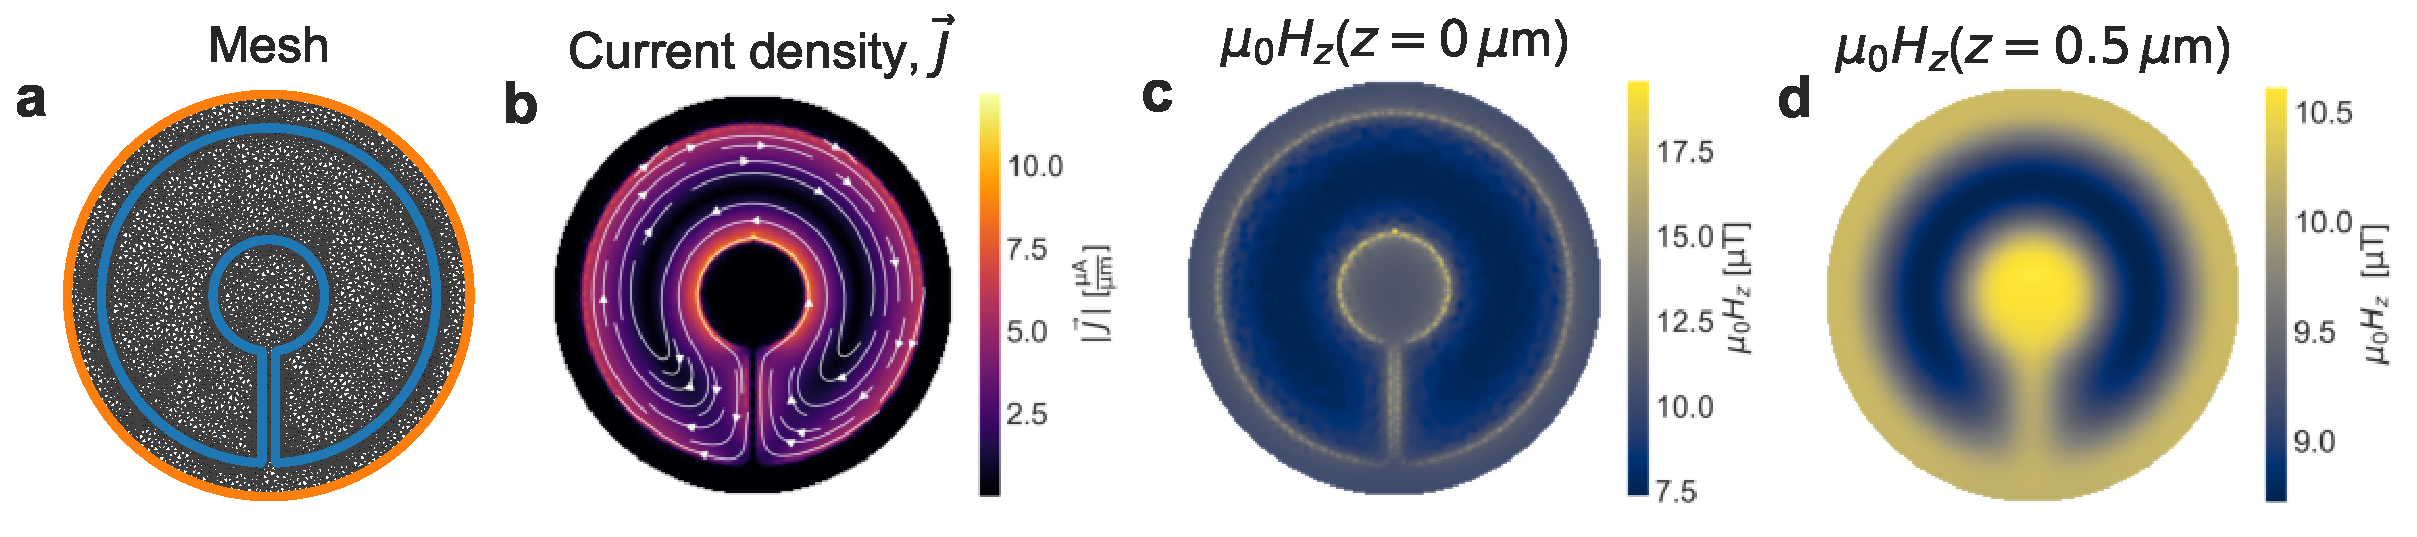
\includegraphics[width=\textwidth]{examples/images/ring_with_slit.pdf}
    \caption{The output of Code Block~\ref{code:device}: Meissner screening of a uniform $10\,\mu\mathrm{T}$ out-of-plane field by a ring with inner diameter $1\,\mu\mathrm{m}$, outer diameter $3\,\mu\mathrm{m}$, and effective penetration depth $\Lambda=1\,\mu\mathrm{m}$, interrupted by a slit of width $0.5\,\mu\mathrm{m}$. a) Plot of the boundary of the ring (blue), circular bounding box (orange), and the computational mesh (gray), generated by \inline{Device.plot()}. b) The $z$-component of the magnetic field $\mu_0H_z$ evaluated at the plane of the ring, generated by \inline{Solution.plot_fields()}. c) Current density $\vec{J}$ in the ring, generated by \inline{Solution.plot_currents()}.}
    \label{fig:ring-with-slit}
\end{figure}

\subsection{Solvers}
\label{section:overview:solvers}

A \SuperScreen model consists of 1) a \inline{Device} with a mesh, 2) a function or \inline{Parameter} that defines the applied magnetic field as a function of position $H_{z,\,\mathrm{applied}}(x, y, z)$, 3) a value for the current circulating around each hole in the device due to trapped flux, and 4) a collection of vortices $v$ located at positions $\vec{r}_v$ and carrying flux $\Phi_v$. These items serve as the inputs to \SuperScreen's main solver function, \inline{superscreen.solve()}, which implements the calculation outlined in Section~\ref{section:implementation}. When simulating a device with more than one layer, one can specify the number of times to implement the iterative calculation described in Section~\ref{section:model:multilayer} in order to solve for the response of all layers self-consistently. One can also skip the iterative portion of the calculation entirely and only solve for the response of each layer to the applied field, assuming no interaction between layers. The \inline{Device.solve_dtype} attribute determines the \inline{numpy} floating point data type used by \inline{solve()}. The default data type is \inline{float64} (64-bit double-precision float, equivalent to Python's \inline{float} type), but one can, for instance, set \inline{device.solve_dtype = "float32"} to use 32-bit single-precision floats in order to save memory.

% \begin{code}
% \begin{minted}[fontsize=\small]{python}
% import numpy as np

% # Simulate the response of the square ring to a uniform applied field of 0.5 mT
% applied_field = sc.sources.ConstantField(0.5)
% field_units = "mT"
% solutions = sc.solve(
%     device=square_ring, applied_field=applied_field, field_units=field_units,
% )
% assert len(solutions) == 1 # Since there is only one layer in this Device
% uniform_field_solution = solutions[-1]

% # Simulate a current circulating around the hole in the ring
% # (with no applied field).
% trapped_flux_solution = sc.solve(
%     device=square_ring, applied_field=None, circulating_currents={"hole" : "1 mA"},
% )[-1]

% # Specify a sequence of (x, y) coordinates to plot cross-sections
% # of the simulated currents and fields.
% xs = np.linspace(-5.5, 5.5, 201) # [microns]
% cross_sections = [ # Two sets of [x, y] coordinates
%     np.stack([xs, xs], axis=1), # diagonal cross-section
%     np.stack([xs, np.zeros_like(xs)], axis=1), # horizontal cross-section
% ]
% for solution in (uniform_field_solution, trapped_flux_solution):
%     solution.plot_currents(cross_section_coords=cross_sections, units="mA/um")
%     solution.plot_fields(cross_section_coords=cross_sections)
% \end{minted}
% \captionof{listing}{Solves for the current and magnetic field distributions for the \inline{square_ring} device given a uniform applied field, and circulating current with no applied field, and plots the resulting sheet current and field.}
% \label{code:ring_circulating_current}
% \end{code}

% Code Block~\ref{code:ring_circulating_current} solves two models involving the \inline{square_ring} device, which was generated using Code Blocks~\ref{code:device} and \ref{code:mesh_generation}. First, Meissner screening of a spatially uniform applied out-of-plane magnetic field and second, the response of the ring to trapped flux with an associated circulating current of 1 mA (with no applied magnetic field). The resulting sheet current and magnetic field distributions (calculated using the optimized mesh shown in Figure~\ref{fig:mesh}d) can be visualized using the \inline{plot_currents()} and \inline{plot_fields()} methods, which produce the images shown in Figure~\ref{fig:square-ring-results}.

% \begin{figure}
%     \centering
%     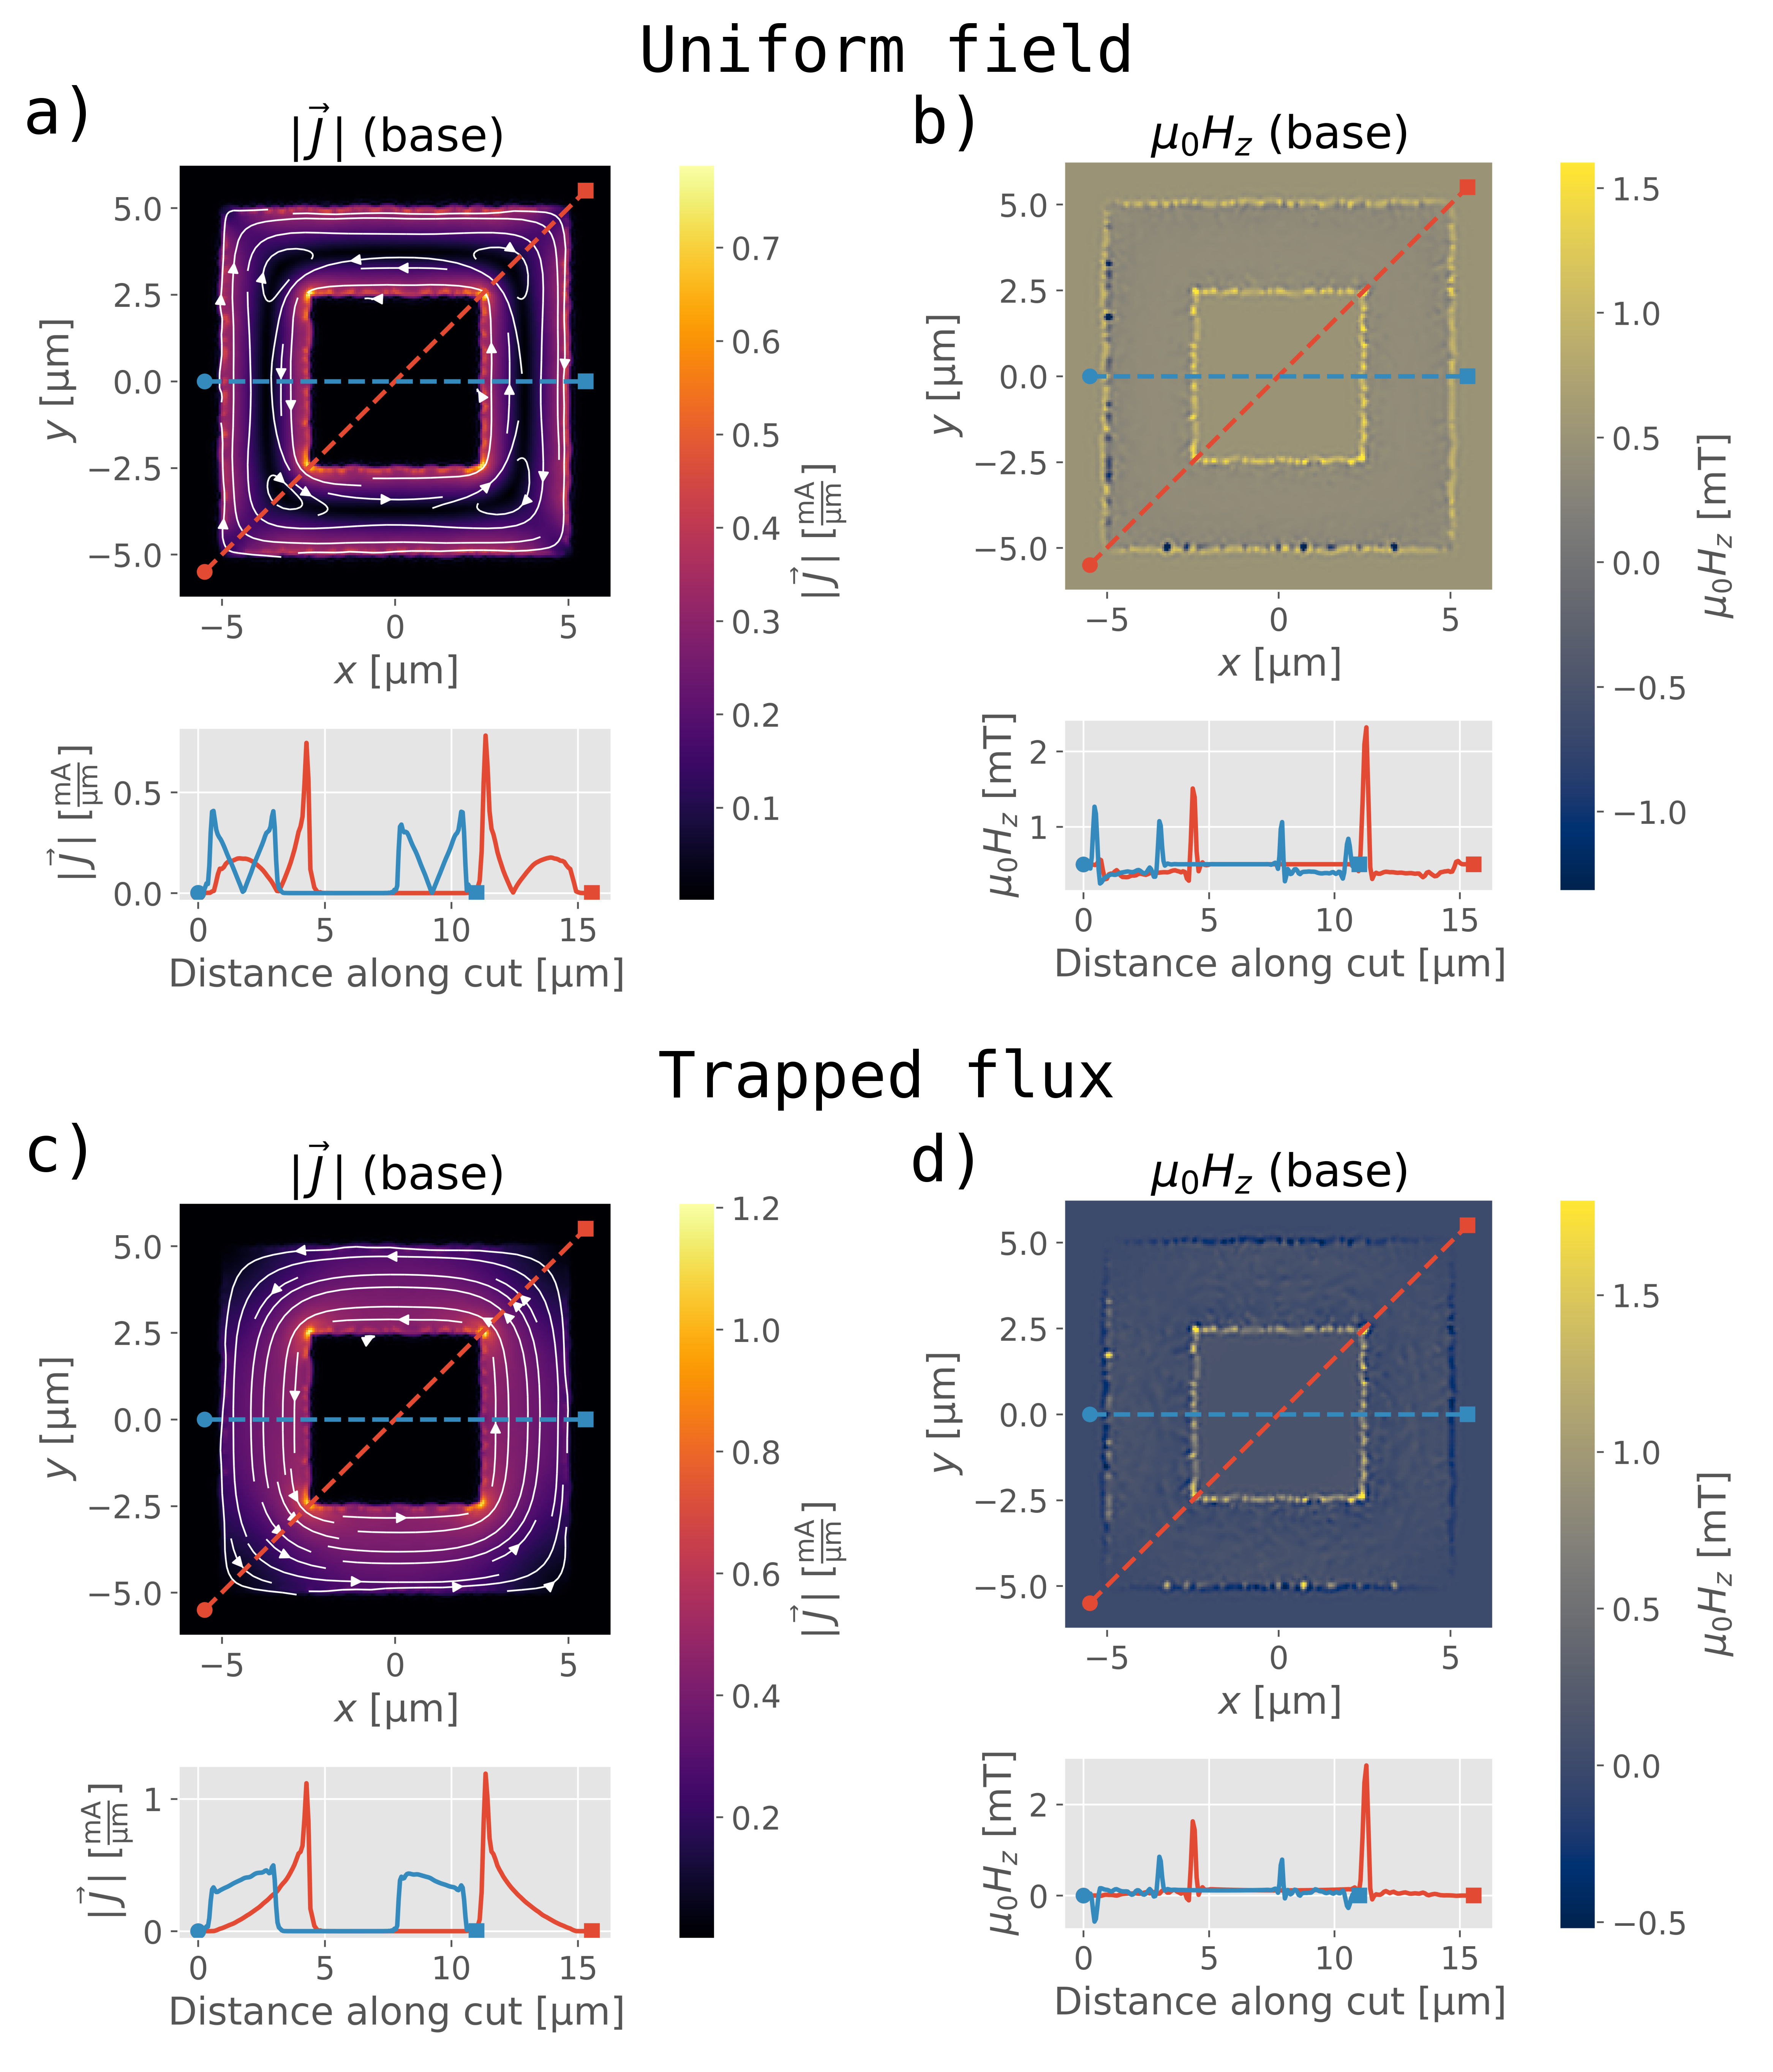
\includegraphics[width=\textwidth]{examples/images/square_ring_results.png}
%     \caption{Sheet current $\vec{J}(x, y)$ and out-of-plane magnetic field $\mu_0H_z(x, y)$ evaluated in the plane of a square ring with effective penetration depth $\Lambda=1\,\mu\mathrm{m}$ subject to (a, b) a uniform applied field of 0.5 mT or (c, d) trapped flux inducing a circulating current of 1 mA. The sub-figures show the output of (a, c) \inline{Solution.plot_currents()} and (b, d) \inline{Solution.plot_fields()}, as shown in Code Block~\ref{code:ring_circulating_current}. For the current plots (a, c), the color-scale indicates the magnitude of the sheet current (or current density), $|\vec{J}|$, and the direction is indicated by the white streamlines.}
%     \label{fig:square-ring-results}
% \end{figure}

The output of \inline{superscreen.solve()} is a \inline{list} of \inline{superscreen.Solution} objects, with a length of 1 plus the number of iterations used for the iterative portion of the calculation. A \inline{Solution} encapsulates all of the information about a solved model: the \inline{Device}, applied field, circulating currents, vortices, and calculated stream functions and magnetic fields for all layers in the device. A \inline{Solution} also has methods for processing the simulation results, including:
\begin{itemize}
    \item{
    \inline{Solution.grid_data()}: Interpolates the calculated stream functions $g(x, y)$, magnetic fields $\mu_0H_z(x, y)$, or current densities $\vec{J}(x, y)$, for each layer from the triangular mesh to a rectangular grid.
    }
    % \item{
    % \inline{Solution.grid_current_density()}: Interpolates the stream functions to a rectangular grid and calculates the current density (sheet current) $\vec{J}(x, y)$ in each layer using Eq.~\ref{eq:stream}.
    % }
    \item{
    \inline{Solution.field_at_position()}: Calculates the vector magnetic field at any point(s) in space due the applied field and the currents flowing the in the device using Eqs.~\ref{eq:field_from_kernel} and \ref{eq:kernels}.
    }
    \item{
    \inline{Solution.interp_current_density()}: Evaluates the current density (sheet current) $\vec{J}(x, y)$ in each layer at arbitrary $(x, y)$ coordinates via interpolation.
    }
    \item{
    \inline{Solution.polygon_flux()}: Calculates the total flux through each polygon in the device (films, holes, and abstract regions).
    }
    \item{
    \inline{Solution.polygon_fluxoid()}: Calculates the fluxoid for a specified polygonal region in the device. See Section~\ref{section:examples:fluxoid} for more details.
    }
\end{itemize}
\inline{Solutions} also have several visualization methods built in (see Section~\ref{section:overview:visualization}).

One may wish to solve many models involving the same device while varying other aspects of the model, for example sweeping the applied field, circulating currents, vortex properties, or some parameter of one or more layers in the device. Fortunately, the mesh and large matrices described in Section~\ref{section:implementation} depend only on the geometry of the device parallel to the $x-y$ plane. This means that the same mesh and matrices can be re-used for models with different applied fields, circulating currents, vortex properties, layer heights (vertical positions), and penetration depths.

The \inline{superscreen.solve_many()} function manages the setup and execution of such a sweep. One can provide a sequence of \inline{Parameter} objects defining different applied fields and/or a sequence of circulating current values over which to sweep and/or a ``layer updater" function that modifies each layer in the device according to some set of keyword arguments, which can also be swept. The latter option can be used to sweep layer heights or penetration depths. Given these inputs, \inline{superscreen.solve_many()} will generate and solve all of the corresponding models. The models can either be solved in series in a single Python process (the default), or in parallel in multiple Python processes running across multiple CPUs, or even across multiple nodes in a cluster (see~\ref{section:parallel}).

\subsection{Visualization}
\label{section:overview:visualization}

\SuperScreen offers several functions for visualizing the results of simulations (which are also aliased as methods on \inline{superscreen.Solution}):

\begin{itemize}
    \item{
    \inline{superscreen.plot_streams()}: Given a \inline{Solution}, plots the stream function $g(x, y)$ for one or more layers in the device.
    
    See also: \inline{Solution.plot_streams()}.
    }
    \item{
    \inline{superscreen.plot_currents()}: Given a \inline{Solution}, plots the sheet current $\vec{J}(x, y)$ for one or more layers in the device.
    
    See also: \inline{Solution.plot_currents()}.
    }
    \item{
    \inline{superscreen.plot_fields()}: Given a \inline{Solution}, plots the total field $H_z(x, y)$ or the screening field $H_z(x, y) - H_{z,\,\mathrm{applied}}(x, y)$ for one or more layers in the device.
    
    See also: \inline{Solution.plot_fields()}.
    }
    \item{
    \inline{superscreen.plot_field_at_positions()}: Given a \inline{Solution}, plots the total field $\vec{H}(x, y, z)$ or $H_z(x, y, z)$ at an arbitrary set of positions $(x, y, z)$.
    
    See also: \inline{Solution.plot_field_at_positions()}.
    }
\end{itemize}

% See Code Block~\ref{code:ring_circulating_current} and  Figure~\ref{fig:square-ring-results} for an example of the usage and output of \inline{plot_fields()} and \inline{plot_currents()}.

\subsection{Comparison \& Persistence}
\label{section:overview:persistence}

\inline{Parameters}, \inline{Layers}, \inline{Polygons}, \inline{Devices}, and \inline{Solutions} all implement the equality operator, \inline{==}. Two \inline{Parameters} are considered equal if the Python bytecode of their underlying functions is the same and their keyword arguments are the same. Two \inline{Layers} are equal if their name, penetration depth, thickness, and vertical position are all equal. Two \inline{Polygons} are equal if they are in the same layer and their name and polygon vertices are equal. Two \inline{Devices} are equal if their name, layers, films, holes, and abstract regions are all equal. Two \inline{Solutions} are equal if their device, applied field, circulating currents, list of trapped vortices, timestamp (time at which the solution was created), and all stream function and magnetic field arrays are equal. Two \inline{Solutions} created at different times can also be compared using the  \inline{solution.equals()} method.

Instances of \inline{superscreen.Device} and \inline{superscreen.Solution} can be saved to and loaded from disk using their respective \inline{to_file()} and \inline{from_file()} methods, making it straightforward to share models and simulation results. \inline{Layers}, \inline{Polygons}, and all metadata are serialized to JSON, a widely-used, human-readable plain text format. Functions and \inline{Parameters}, such as those that compute the applied field or penetration depth, are serialized in binary form using \inline{dill}~\cite{McKerns}. \inline{Numpy} arrays, such as the mesh itself and the computed stream functions and fields, are saved in the \inline{numpy} \inline{npz} file format. A \inline{list} of \inline{Solutions}, such as that returned by \inline{superscreen.solve()} can be saved/loaded all at once using \inline{save_solutions()} and \inline{load_solutions()}.

% \section{Example application: Scanning SQUID magnetometry}
% \label{section:application}
% In scanning superconducting quantum interference device (SQUID) susceptometry, the diamagnetic susceptibility of a superconducting sample is measured by bringing the sample close to a pair of superconducting loops. The first loop, called the ``pickup loop" is attached to a SQUID circuit that sensitively measures the magnetic flux threading the loop. The second loop, called the ``field coil," carries a known current and applies a known magnetic field to both the pickup loop and the sample. The superconducting sample screens the magnetic field from the field coil, modifying the amount of flux threading the pickup loop. Thus the mutual inductance between the field coil and pickup loop provides a measure of the sample's diamagnetic susceptibility, which is in turn a measure of the sample's penetration depth.

% Analysis developed to interpret the results of scanning SQUID susceptometry measurements makes several simplifying assumptions that are not always satisfied: 1) the sample's effective penetration depth $\Lambda$ (or Pearl length $2\Lambda$) is spatially homogeneous, 2) the sample is much larger than the field coil, and 3) the field coil and pickup loop can be approximated as one-dimensional coaxial, coplanar circular loops~\cite{Kirtley_Kalisky_2012}.

% \begin{figure}[!h]
% \centering
% \begin{subfigure}{.35\textwidth}
%   \centering
%   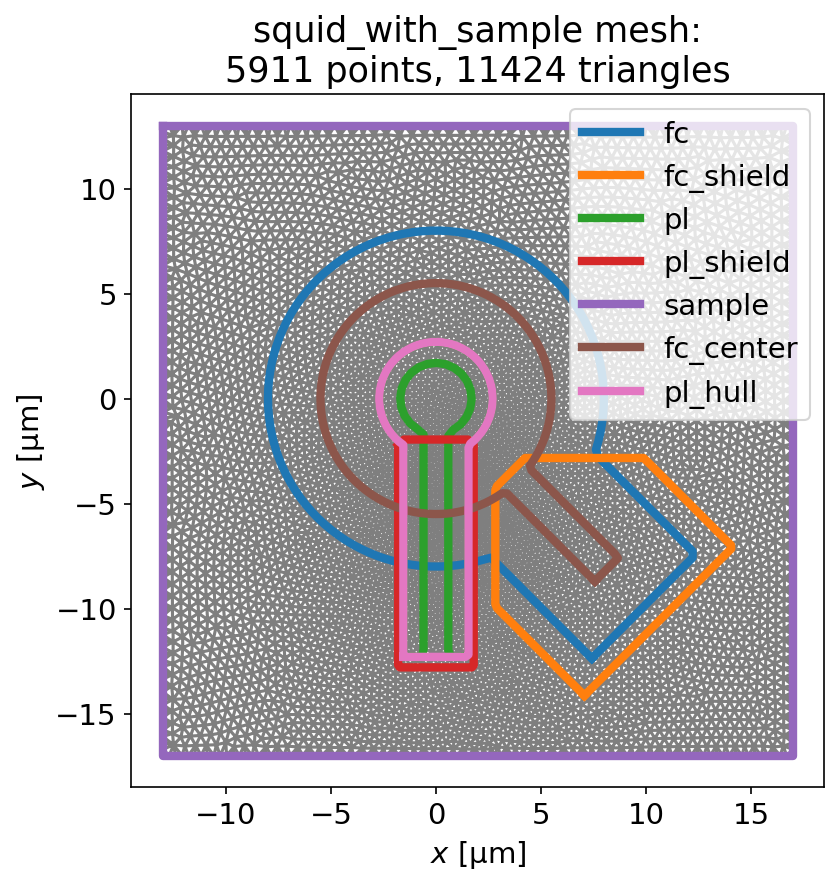
\includegraphics[width=\linewidth]{examples/images/squid_susceptometry/squid_with_sample_mesh.png}
%   \label{fig:squid_mesh}
%   \caption{}
% \end{subfigure}%
% \hspace{10pt}
% \begin{subfigure}{.5\textwidth}
%   \centering
%   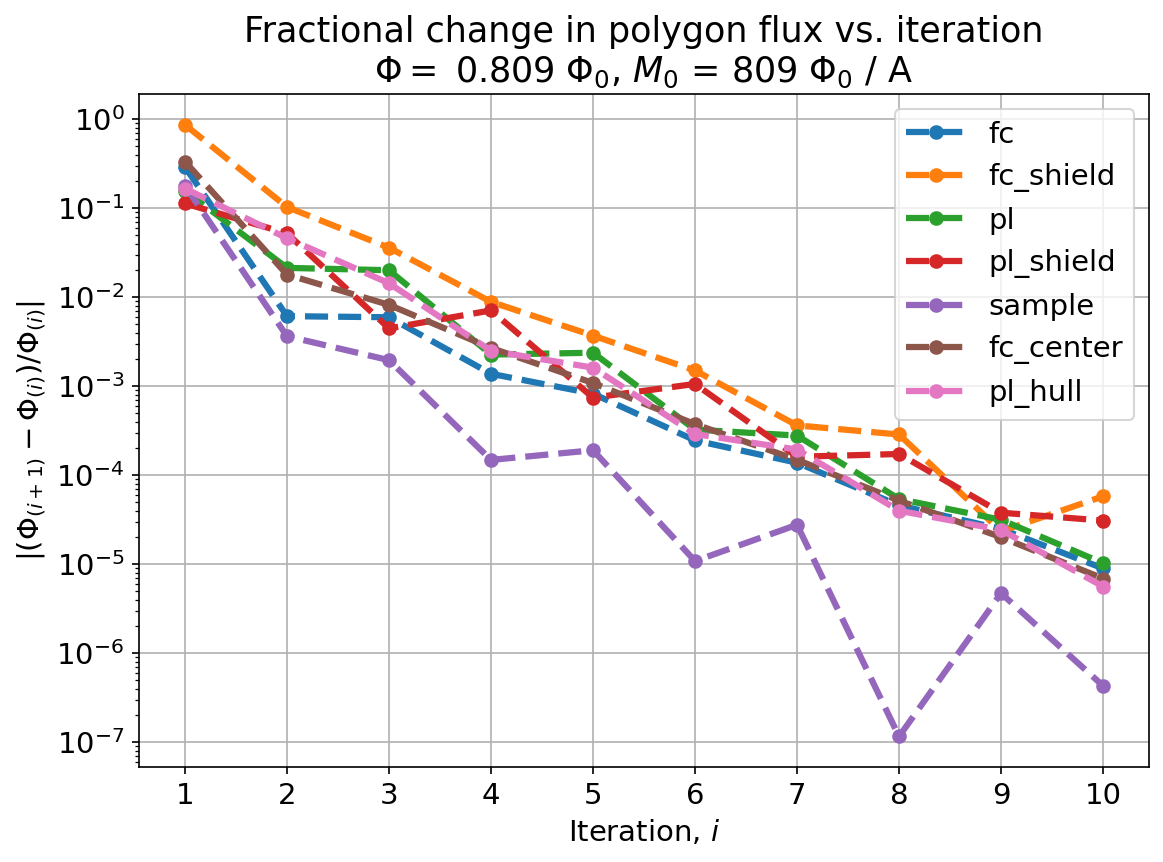
\includegraphics[width=\linewidth]{examples/images/squid_susceptometry/squid_with_sample_M0_convergence.png}
%   \label{fig:squid_convergence}
%   \caption{}
% %   \caption{Fractional change in flux though all polygons vs. solver iteration with a current of $1\,\mathrm{mA}$ flowing in the field coil (\inline{fc}). The mutual inductance $M_0$ is given by the flux through the pickup loop (\inline{pl_hull}) divided by the field coil current.}
% \end{subfigure}%
% \caption{(a): Device polygons and mesh for the SQUID susceptometer model. (b) Fractional change in flux though all polygons vs. solver iteration with a current of $1\,\mathrm{mA}$ flowing in the field coil (\inline{fc}). The mutual inductance $M_0$ is given by the flux through the pickup loop (\inline{pl_hull}) divided by the field coil current.}
% \label{fig:susceptometry}
% \end{figure}

% Figure~\ref{fig:susceptometry}(a) shows a \inline{Device} representing field coil and pickup loop of an actual scanning SQUID sensor. In addition to the field coil and pickup loop, there are superconducting shields that limit the amount of magnetic flux that can penetrate the leads connecting the loops to the rest of the circuit (the rest of the circuit is not modeled). There are three relevant layers of superconducting films: the base electrode (``BE"), which is furthest from the sample contains the field coil; the first wiring layer (``W1"), which contains the pickup loop and a shield covering the field coil leads; and the second wiring layer (``W2"), which is closest to the sample and contains a shield covering the pickup loop leads. The device also contains a layer and film representing the superconducting sample.

% To model a SQUID susceptometry measurement, we first calculate $M_0$, the mutual inductance between the field coil and pickup loop in the absence of the sample. This can be done by temporarily setting the sample layer effective penetration depth to a very large value such that it essentially does not screen the field from the field coil (in this case, we set $\Lambda = 10^5\,\mu\mathrm{m}$). We then model the field from a known current flowing in the field coil following Section~\ref{section:model:holes} and self-consistently calculate the response of both the sample and the other superconducting layers of the SQUID sensor following Section~\ref{section:model:multilayer}. To ensure that the 2D current distribution in the field coil is approximately uniform (as we would expect for a real applied current), we set the field coil layer effective penetration depth to be greater than the width of the field coil conductor.

% Once $M_0$ is known, we can ``turn on" the sample's diamagnetic response by setting its effective penetration depth $\Lambda$ to the desired value and compute $M(z, \Lambda)$ for a given vertical distance $z$ between the sample and the SQUID as described in the previous paragraph. The SQUID susceptibility signal is then $M(z, \Lambda) - M_0$, the change in mutual inductance between the field coil and pickup loop due to the presence of the sample (usually given in units of $\Phi_0/\mathrm{A}$, where $\Phi_0$ is the superconducting flux quantum). The susceptibility can also be normalized to the bare mutual inductance $M_0$, giving a dimensionless susceptibility $\chi(z, \Lambda)=[M(z, \Lambda) - M_0] / M_0$.  

% % \begin{figure}[!h]
% % \centering
% % \begin{subfigure}{\textwidth}
% %   \centering
% %   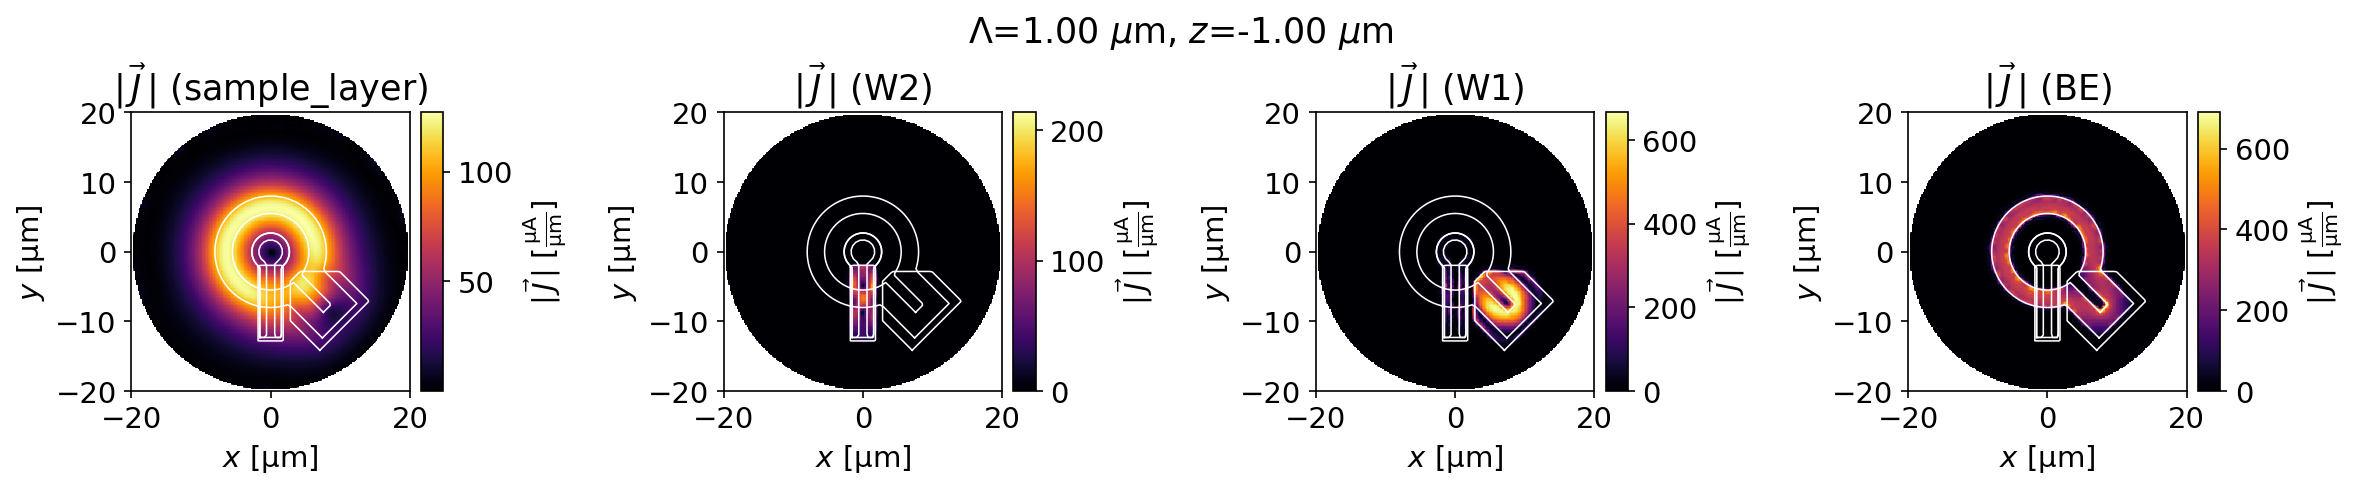
\includegraphics[width=\linewidth]{examples/images/squid_susceptometry/squid_with_sample_currents_Lambda=1_00__um__z=-1_00__um.png}
% % %   \caption{Device polygons and mesh for the SQUID susceptometer model.}
% % %   \label{fig:squid_mesh}
% % \end{subfigure}%
% % \vspace{-15pt}
% % \begin{subfigure}{\textwidth}
% %   \centering
% %   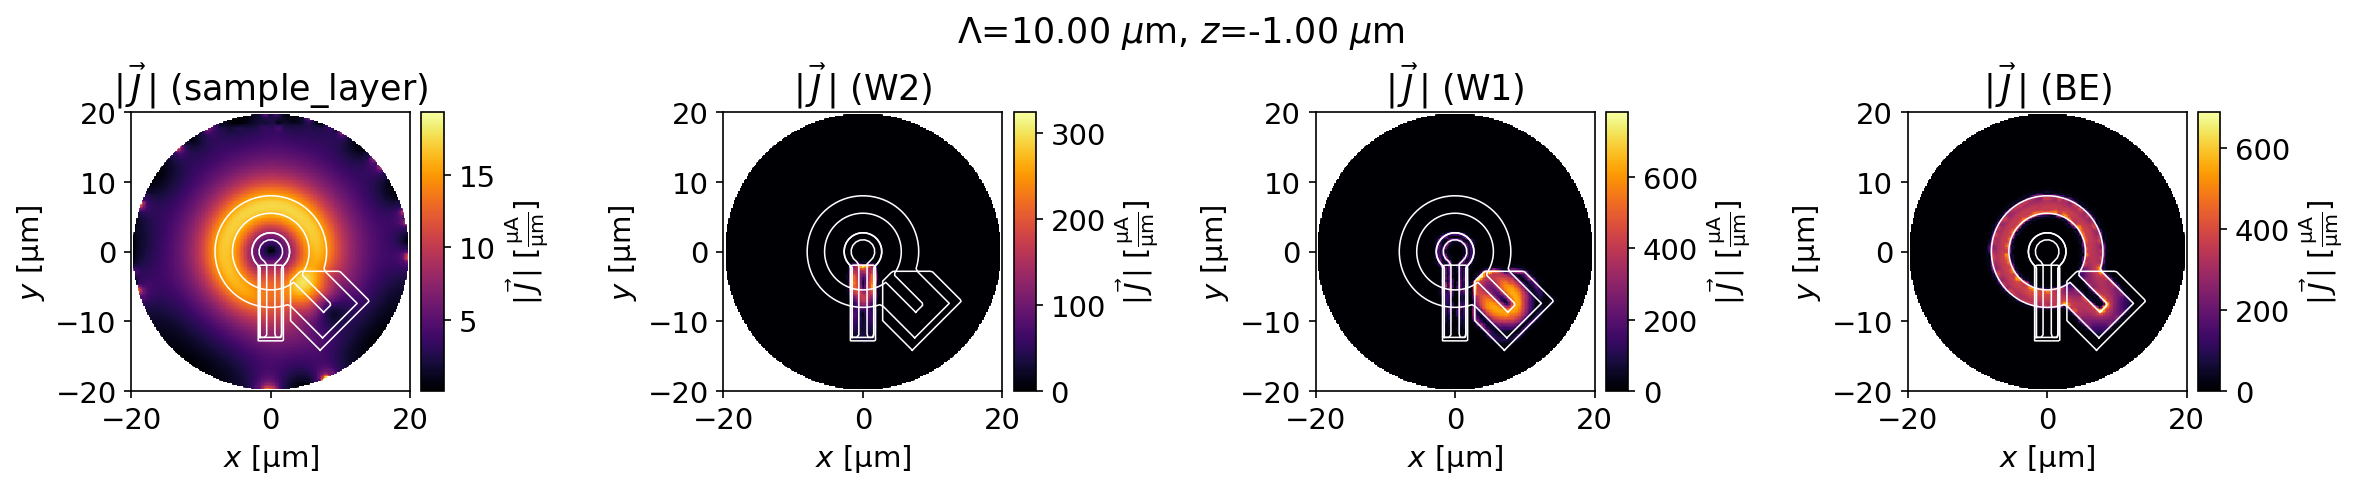
\includegraphics[width=\linewidth]{examples/images/squid_susceptometry/squid_with_sample_currents_Lambda=10_00__um__z=-1_00__um.png}
% % %   \caption{Fractional change in flux though all polygons vs. solver iteration with a current of $1\,\mathrm{mA}$ flowing in the field coil (\inline{fc}). The mutual inductance $M_0$ is given by the flux through the pickup loop (\inline{pl_hull}) divided by the field coil current.}
% % %   \label{fig:squid_convergence}
% % \end{subfigure}%
% % \vspace{-15pt}
% % \begin{subfigure}{\textwidth}
% %   \centering
% %   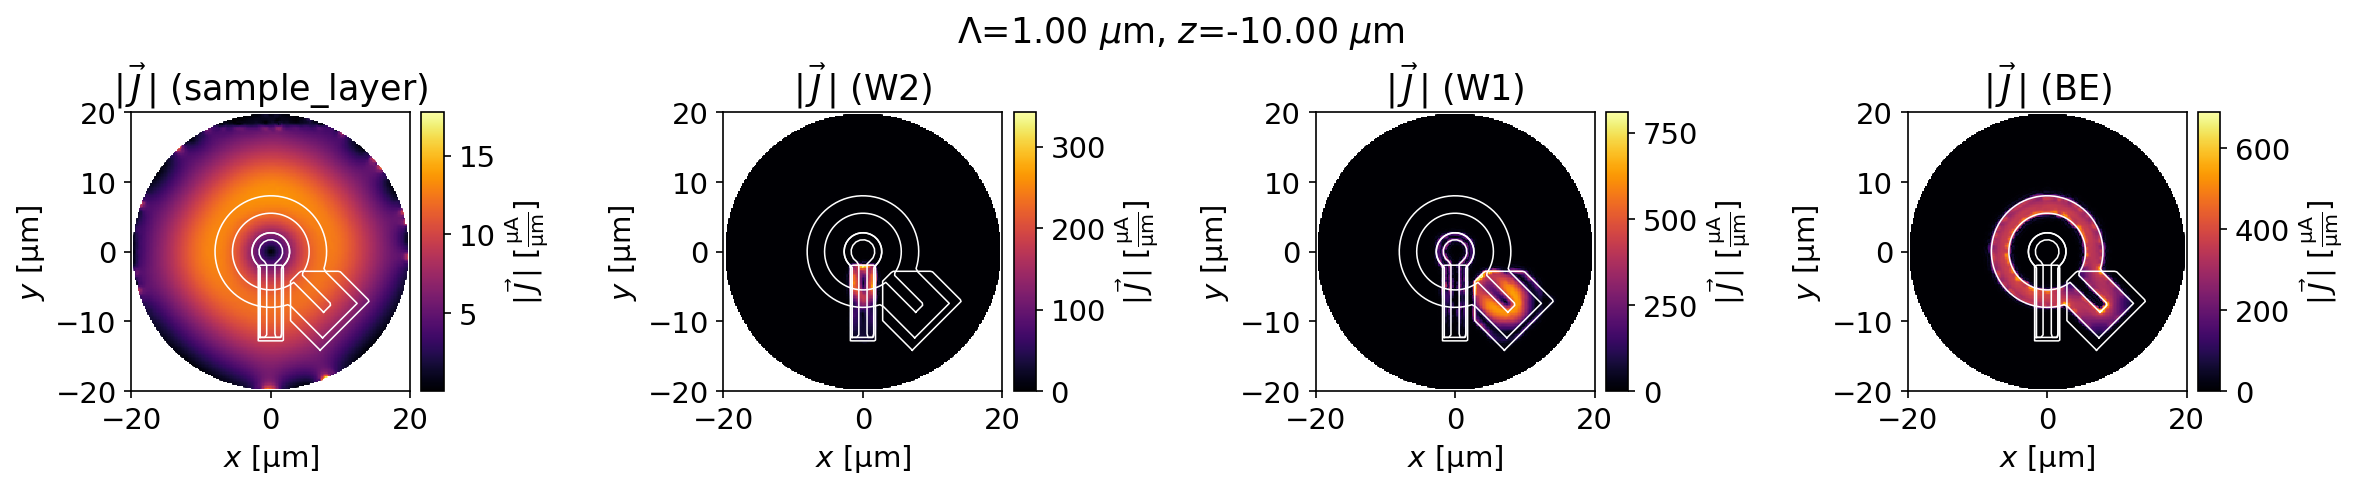
\includegraphics[width=\linewidth]{examples/images/squid_susceptometry/squid_with_sample_currents_Lambda=1_00__um__z=-10_00__um.png}
% % %   \caption{Fractional change in flux though all polygons vs. solver iteration with a current of $1\,\mathrm{mA}$ flowing in the field coil (\inline{fc}). The mutual inductance $M_0$ is given by the flux through the pickup loop (\inline{pl_hull}) divided by the field coil current.}
% % %   \label{fig:squid_convergence}
% % \end{subfigure}%
% % \caption{Left: Device polygons and mesh for the SQUID susceptometer model. Right: Fractional change in flux though all polygons vs. solver iteration with a current of $1\,\mathrm{mA}$ flowing in the field coil (\inline{fc}). The mutual inductance $M_0$ is given by the flux through the pickup loop (\inline{pl_hull}) divided by the field coil current.}
% % % \label{fig:susceptometry}
% % \end{figure}

\section{Examples}
\label{section:examples}

\subsection{Pearl vortices in thin films}
\label{section:examples:pearl-vortices}
Vortices trapped in 2D superconductors ($d\ll\lambda$, where $d$ is the film thickness and $\lambda$ is the London penetration depth), i.e. ``Pearl vortices,'' are associated with different current and magnetic field distributions than Abrikosov vortices trapped in bulk type-II superconductors~\cite{Pearl1964-cl}. The 2D Fourier transform $\tilde{H}_z(\vec{k}, z)$ of the out-of-plane component of the magnetic field $H_z(\vec{r}, z)$ from a Pearl vortex located at the origin $x=y=z=0$ is given by

\begin{equation}
    \tilde{H}_z(\vec{k}, z)=\mathcal{F}\{H_z(\vec{r}, z)\}=\frac{1}{\mu_0}\frac{\Phi_0e^{-|\vec{k}|z}}{1+2\Lambda|\vec{k}|},
    \label{eq:pearl}
\end{equation}
where $\mathcal{F}\{\cdot\}$ is the 2D Fourier transform, $\vec{k}=(k_x, k_y)$ are in-plane spatial frequencies, $z$ is the out-of-plane position at which the field is evaluated, and $2\Lambda = 2\lambda^2 / d$ is the Pearl length~\cite{Pearl1964-cl, Tafuri2004-ap}. The real-space magnetic field distribution near a Pearl vortex can be calculated numerically by taking the inverse Fourier transform of Eq.~\ref{eq:pearl}: $H_z(\vec{r}, z)=\mathcal{F}^{-1}\{\tilde{H}_z(\vec{k}, z)\}$. The field distributions generated by \SuperScreen in the presence of vortices as described in Sections~\ref{section:model:vortices} and~\ref{section:implementation} agree to within a few percent with the distributions obtained using this Fourier transform method, as demonstrated in Code Block~\ref{code:pearl-vortex} and Figure~\ref{fig:pearl}(c-e).

To include vortices in a \SuperScreen model, one can simply input a \inline{list} of \inline{superscreen.Vortex} objects when calling \inline{superscreen.solve()} (see Code Block~\ref{code:pearl-vortex}). A \inline{Vortex} object specifies the $x,y$ position for the vortex core, the name of the superconducting layer in which the vortex is pinned, and the number of flux quanta $\Phi_0$ contained in the vortex (which is 1 by default). See Ref.~\cite{Brandt2005-wj} for a method to compute the self-energy and interaction energies of vortices in thin films.

\begin{code}
\begin{minted}[fontsize=\small]{python}
# Create a device representing square thin film.
device = sc.Device(
    "film",
    layers=[sc.Layer("base", Lambda=0, z0=0)],
    films=[sc.Polygon("film", layer="base", points=sc.geometry.square(20))],
    length_units="um",
)
device.make_mesh(min_triangles=8000)
# Specify the vortex position.
vortices = [sc.Vortex(x=0, y=0, layer="base")]
# Sweep Lambda, solve the model, and evaluate the field at the given coordinates.
Lambdas = np.linspace(0, 2, 5) # [device.length_units]
for Lambda in Lambdas:
    device.layers["base"].Lambda = Lambda
    solution = sc.solve(device=device, vortices=vortices)[-1]
    # Use solution.field_at_position() to evaluate the magnetic field profile,
    # and solution.polygon_fluxoid() to calculate fluxoids.
\end{minted}
\captionof{listing}{Creates a square superconducting film with side length $20\,\mu\mathrm{m}$ and calculates the magnetic field distribution near a vortex at the center of the film as a function of the the effective penetration depth, $\Lambda$ (see Figure~\ref{fig:pearl}).}
\label{code:pearl-vortex}
\end{code}

\begin{figure}[h]
    \centering
    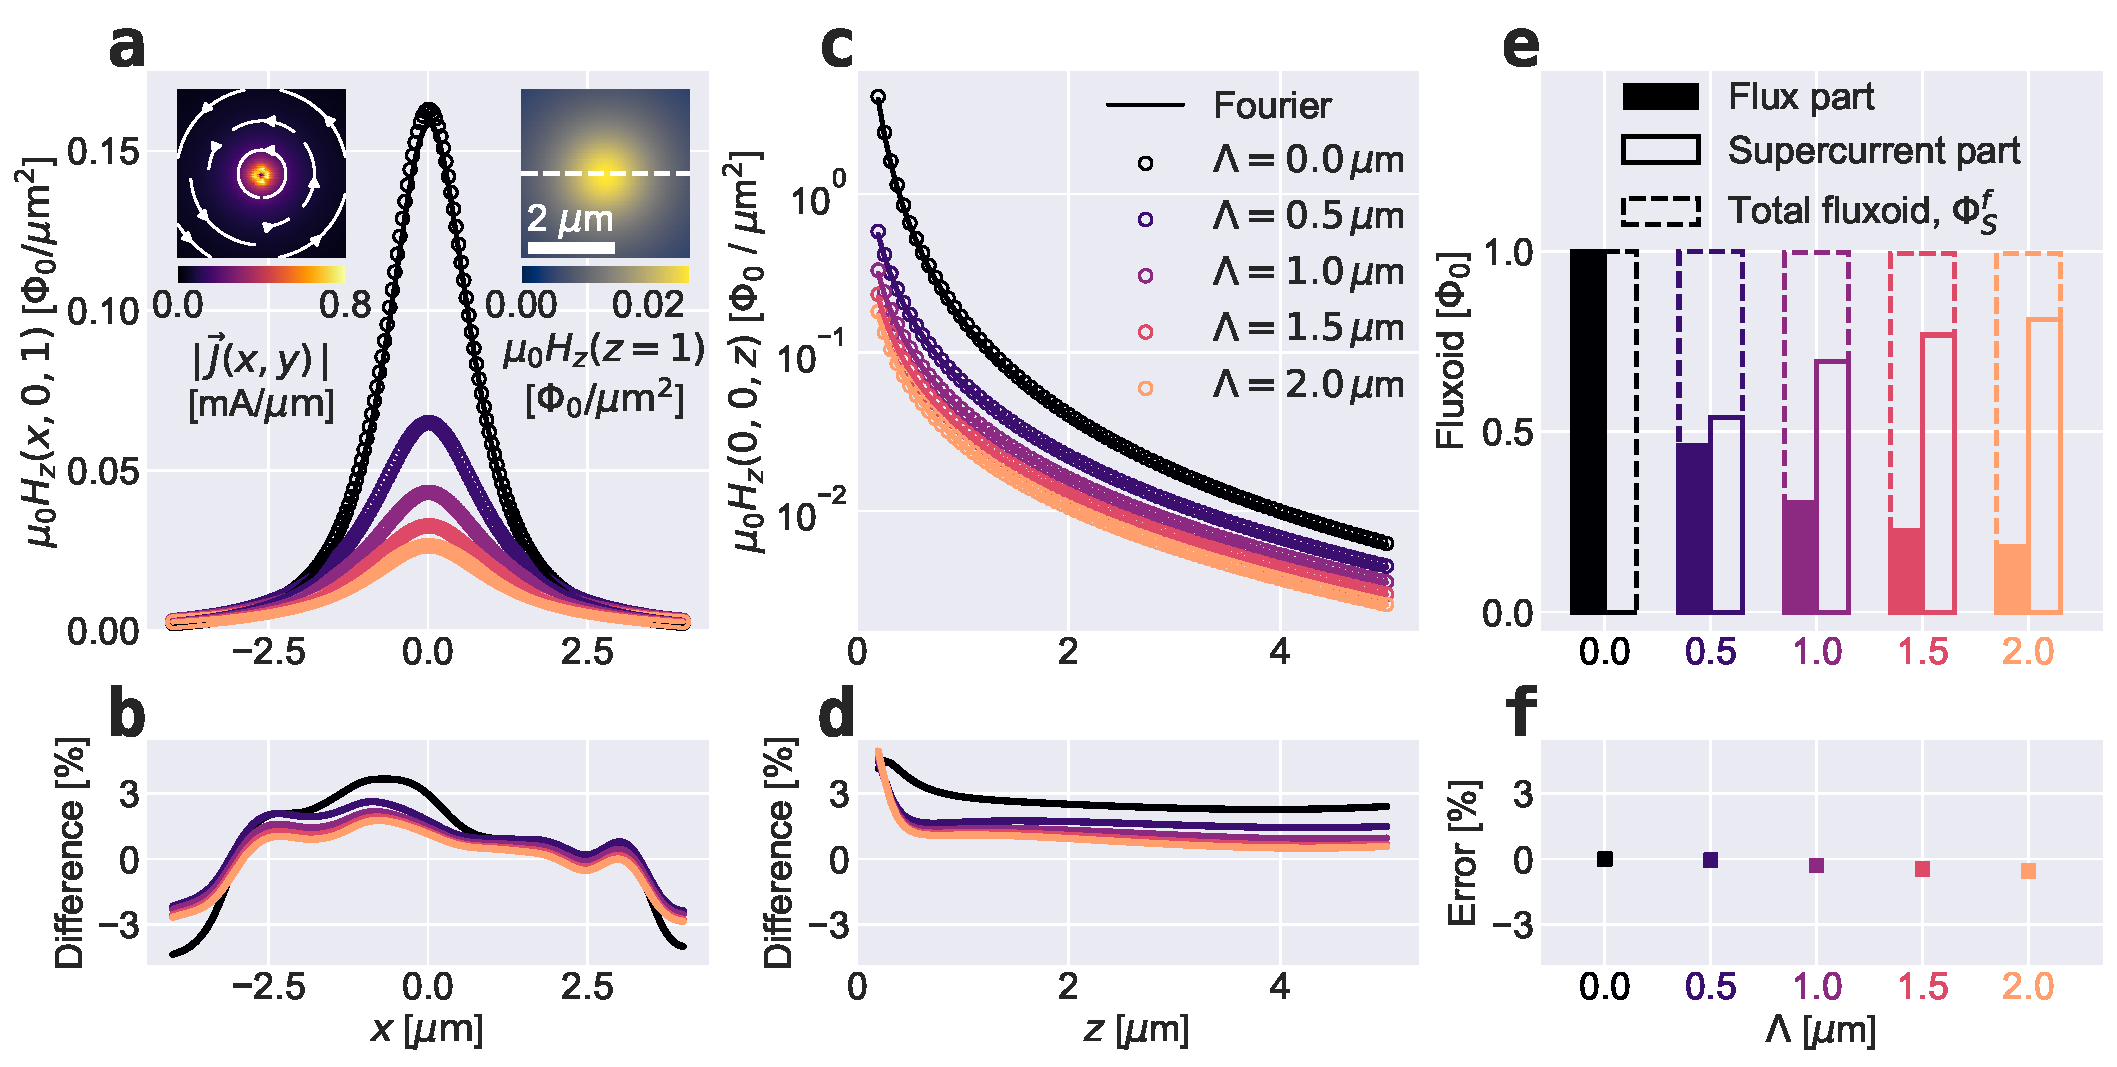
\includegraphics[width=\textwidth]{examples/images/pearl.pdf}
    \caption{Vortex field profiles calculated with \SuperScreen agree with the analytical solution (Eq.~\ref{eq:pearl}) to within a few percent. Here, we model a vortex trapped at the center of a square superconducting film lying in the $x-y$ plane with side length $20\,\mu\mathrm{m}$ as a function of the film's effective penetration depth, $\Lambda$. (a) Cross section along the $x$-axis of the out-of-plane magnetic field $\mu_0H_z$ from the vortex, evaluated at a vertical distance $z=1\,\mu\mathrm{m}$ above the film. (b) Percentage difference between the $\mu_0H_z$ calculated with \SuperScreen and the Fourier transform method for the $x$-axis cut shown in (a). (c) Cross-section along the $z$-axis of $\mu_0H_z$ directly above the center of the vortex (logarithmic $y$ axis scale). (d) Percentage difference between the $\mu_0H_z$ calculated with \SuperScreen and the Fourier transform method for the $z$-axis cut shown in (c). In (a) and (c), the results from \SuperScreen are shown as open circles and the results from the Fourier transform method are shown as solid lines. (e) The fluxoid $\Phi_S^f$ for a circular region in the film with radius $r=1\,\mu\mathrm{m}$ centered on the vortex core. As $\Lambda$ increases, so to does the supercurrent contribution to the fluxoid. (f) Error in the total simulated fluxoid relative to $\Phi_0$: $(\Phi_S^f(\Lambda) - \Phi_0) / \Phi_0$.}
    \label{fig:pearl}
\end{figure}

\subsection{Calculating the fluxoid}
\label{section:examples:fluxoid}

\SuperScreen allows one to calculate the fluxoid $\Phi^f_S$ for any polygonal region $S$ whose boundary $\partial S$ lies completely within a superconducting film using the method \inline{Solution.polygon_fluxoid()} (see Section~\ref{section:model:fluxoid}, Eq.~\ref{eq:fluxoid}). The ``flux part''  $\int_S\mu_0H_z(\vec{r})\,\mathrm{d}^2r$ is calculated using \inline{Solution.polygon_flux()}, which computes the flux through a polygon representing a region $S$ by averaging the field at the three vertices of each triangle $t$ whose centroid lies in $S$ to estimate the field $\mu_0H_{z, t}$ at the centroid of the triangle, then returns the flux $\sum_t \mu_0H_{z,t}A_t$, where $A_t$ is the area of triangle $t$. The ``supercurrent part'' $\oint_S\mu_o\Lambda(\vec{r})\vec{J}(\vec{r})\cdot\mathrm{d}\vec{r}$ is calculated by evaluating the vector current density $\vec{J}$ at each point in the path $\partial S$ using \inline{Solution.interp_current_density()}, then computing the line integral along the path using the trapezoid rule. The sum of these two terms gives the fluxoid $\Phi^f_S$.

Figure~\ref{fig:pearl}(e) shows the fluxoid for a circular region $S$ with radius $r=1\,\mu\mathrm{m}$ enclosing a Pearl vortex trapped in a film as a function of the film's effective penetration depth, $\Lambda$. When $\Lambda=0$, the screening currents decay very quickly away from the center of the vortex, so the ``supercurrent part'' of the $\Phi^f_S$ vanishes. With increasing $\Lambda$, the ``supercurrent part'' accounts for an increasing fraction of the total fluxoid.
% See \ref{appendix:fluxoid} for a demonstration of the fluxoid properties listed in Section~\ref{section:model:fluxoid}.

While the 2D London model doesn't ``know'' about fluxoid quantization, in the sense that it is not automatically satisfied by solutions to Eq.~\ref{eq:london} for multiply-connected films, we can nevertheless calculate current and field distributions for different fluxoid states $\Phi^f_S=n\Phi_0$ in multiply-connected superconductors by adjusting the currents circulating around each hole to realize a prescribed set of fluxoid values. For a structure with $N_h$ holes, we can specify $N_h$ fluxoids $\Phi^f_h$ and find the circulating currents $I_h$ by minimizing the deviation of each fluxoid from its desired value. (If $N_h=1$, this is a simple 1D root-finding problem.) This calculation is implemented in the \inline{superscreen.find_fluxoid_solution()} function.

Here, we use \inline{superscreen.find_fluxoid_solution()} to compute the current and field distributions in and around a film with a single hole in the $n=1$ fluxoid state as a function of the film's effective penetration depth, $\Lambda$.

\subsection{Self-inductance and mutual inductance}
\label{section:examples:mutual-inductance}

As shown in Ref.~\cite{Brandt2005-wj}, the mutual inductance $M_{ij}$ between holes $i$ and $j$ in a superconducting structure is given by
\begin{equation}
    M_{ij}=\frac{\Phi^f_{S_i}}{I_j},
\end{equation}
where $\Phi^f_{S_i}$ is the fluxoid for a region $S_i$ containing the hole $i$, and $I_j$ is the current circulating around hole $j$. The mutual inductance values for a set of holes form a mutual inductance matrix. The diagonals of the mutual inductance matrix are the hole self-inductances ($M_{ii}=L_i$, the self-inductance of hole $i$), and the matrix is symmetric ($M_{ij}=M_{ji}$) due to the reciprocity theorem. If the penetration depth of the film containing hole $i$ is $\Lambda = 0$, then no field penetrates the film and the fluxoid $\Phi^f_{S_i}$ is equal to $\Phi_i$, the flux through hole $i$.

We'll focus first on the self-inductance of circular and square rings. For a circular ring with inner radius $a$, outer radius $b>a$, and penetration depth $\Lambda=0$, Clem~\cite{Babaei_Brojeny2003-la} found that the self-inductance approaches $L=2\mu_0 a$ in the ``small hole'' limit $\tilde{a}=a/b\ll 1$. In the opposite ``thin ring'' limit $\tilde{a}=a/b\approx 1$, the inductance was found to approach $L=\mu_0b(1+\tilde{a})(\tanh^{-1}\tilde{a}+\log 4 - 1)$. Clem and Brandt~\cite{Brandt2004-ew} and Khapaev~\cite{Khapaev1997-kw} calculated the self-inductance of circular and square rings as a function of the ratio of inner and outer diameters.

\subsection{Application: scanning SQUID microscopy}
\label{section:examples:scanning-squid}

In scanning superconducting quantum interference device (SQUID) susceptometry, the diamagnetic susceptibility of a superconducting sample is measured by bringing the sample close to a pair of superconducting loops. The first loop, called the ``pickup loop" is attached to a SQUID circuit that sensitively measures the magnetic flux threading the loop. The second loop, called the ``field coil," carries a known current and applies a known magnetic field to both the pickup loop and the sample. The superconducting sample screens the magnetic field from the field coil, modifying the amount of flux threading the pickup loop. Thus the mutual inductance between the field coil and pickup loop provides a measure of the sample's diamagnetic susceptibility, which is in turn a measure of the sample's penetration depth.

Analysis developed to interpret the results of scanning SQUID susceptometry measurements makes several simplifying assumptions that are not always satisfied: 1) the sample's effective penetration depth $\Lambda$ (or Pearl length $2\Lambda$) is spatially homogeneous, 2) the sample is much larger than the field coil, and 3) the field coil and pickup loop can be approximated as one-dimensional coaxial, coplanar circular loops~\cite{Kirtley_Kalisky_2012}.

% \begin{figure}[!h]
% \centering
% \begin{subfigure}{.35\textwidth}
%   \centering
%   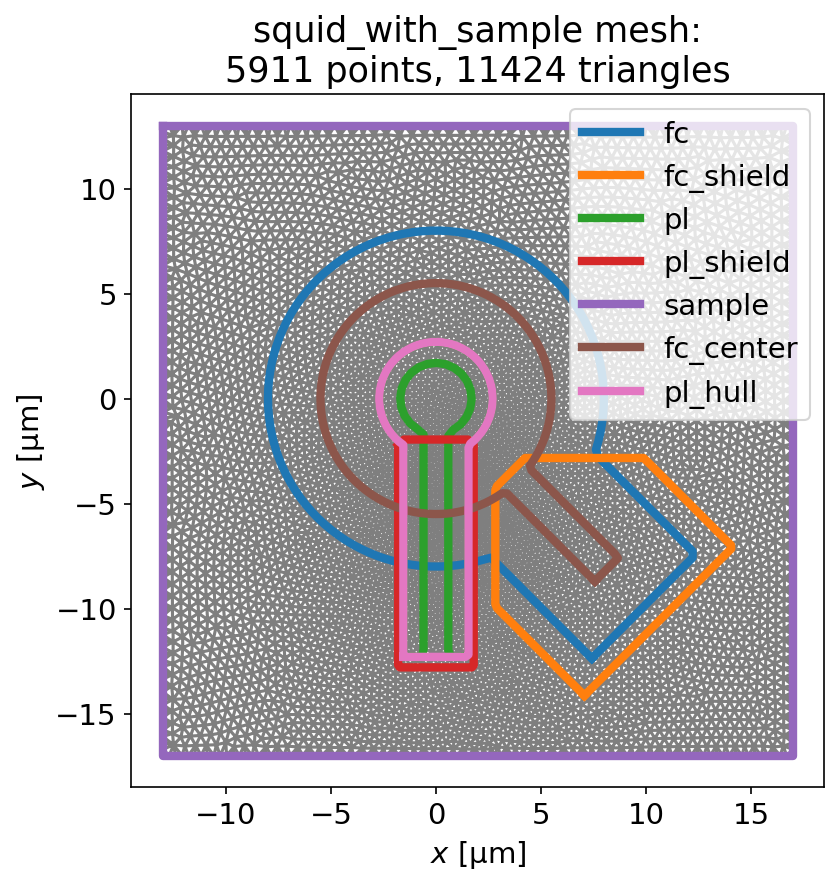
\includegraphics[width=\linewidth]{examples/images/squid_susceptometry/squid_with_sample_mesh.png}
%   \label{fig:squid_mesh}
%   \caption{}
% \end{subfigure}%
% \hspace{10pt}
% \begin{subfigure}{.5\textwidth}
%   \centering
%   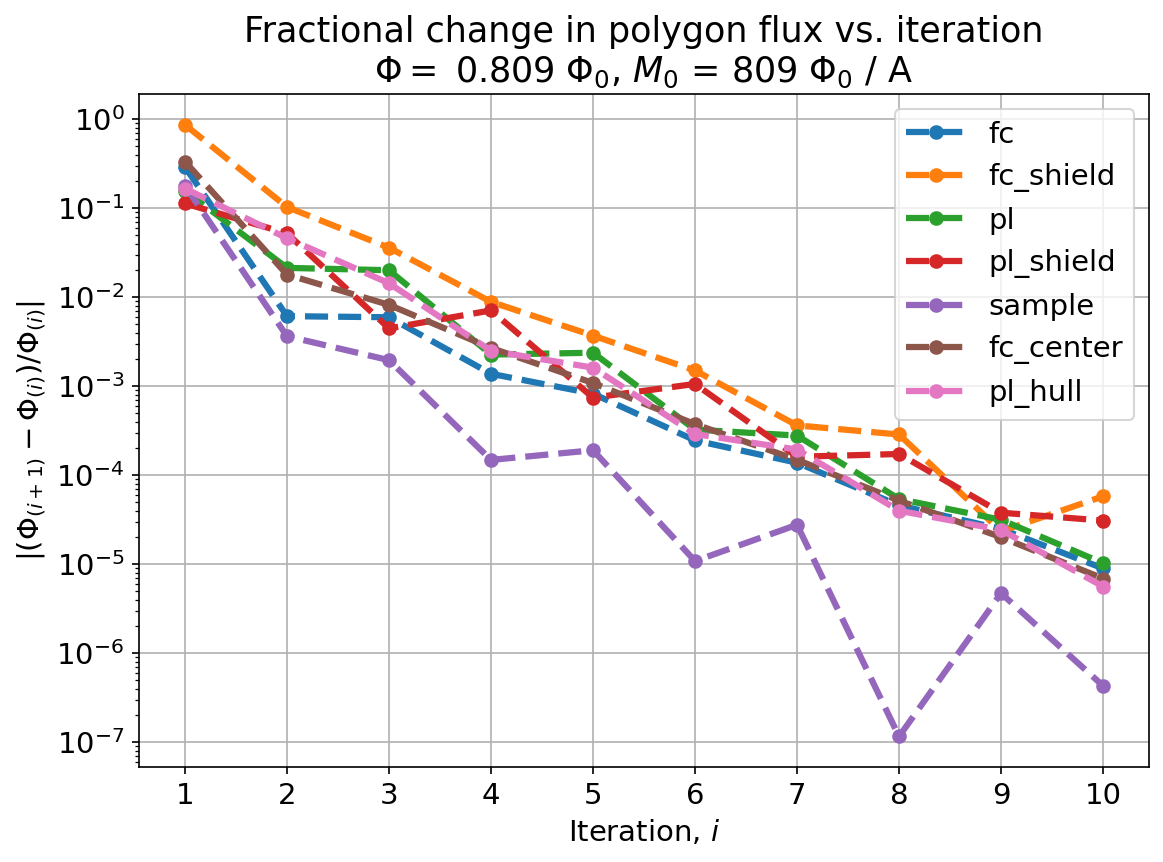
\includegraphics[width=\linewidth]{examples/images/squid_susceptometry/squid_with_sample_M0_convergence.png}
%   \label{fig:squid_convergence}
%   \caption{}
%   \caption{Fractional change in flux though all polygons vs. solver iteration with a current of $1\,\mathrm{mA}$ flowing in the field coil (\inline{fc}). The mutual inductance $M_0$ is given by the flux through the pickup loop (\inline{pl_hull}) divided by the field coil current.}
% \end{subfigure}%
% \caption{(a): Device polygons and mesh for the SQUID susceptometer model. (b) Fractional change in flux though all polygons vs. solver iteration with a current of $1\,\mathrm{mA}$ flowing in the field coil (\inline{fc}). The mutual inductance $M_0$ is given by the flux through the pickup loop (\inline{pl_hull}) divided by the field coil current.}
% \label{fig:susceptometry}
% \end{figure}

Figure~\ref{fig:susceptometry}(a) shows a \inline{Device} representing field coil and pickup loop of an actual scanning SQUID sensor. In addition to the field coil and pickup loop, there are superconducting shields that limit the amount of magnetic flux that can penetrate the leads connecting the loops to the rest of the circuit (the rest of the circuit is not modeled). There are three relevant layers of superconducting films: the base electrode (``BE"), which is furthest from the sample contains the field coil; the first wiring layer (``W1"), which contains the pickup loop and a shield covering the field coil leads; and the second wiring layer (``W2"), which is closest to the sample and contains a shield covering the pickup loop leads. The device also contains a layer and film representing the superconducting sample.

To model a SQUID susceptometry measurement, we first calculate $M_0$, the mutual inductance between the field coil and pickup loop in the absence of the sample. This can be done by temporarily setting the sample layer effective penetration depth to a very large value such that it essentially does not screen the field from the field coil (in this case, we set $\Lambda = 10^5\,\mu\mathrm{m}$). We then model the field from a known current flowing in the field coil following Section~\ref{section:model:holes} and self-consistently calculate the response of both the sample and the other superconducting layers of the SQUID sensor following Section~\ref{section:model:multilayer}. To ensure that the 2D current distribution in the field coil is approximately uniform (as we would expect for a real applied current), we set the field coil layer effective penetration depth to be greater than the width of the field coil conductor.

Once $M_0$ is known, we can ``turn on" the sample's diamagnetic response by setting its effective penetration depth $\Lambda$ to the desired value and compute $M(z, \Lambda)$ for a given vertical distance $z$ between the sample and the SQUID as described in the previous paragraph. The SQUID susceptibility signal is then $M(z, \Lambda) - M_0$, the change in mutual inductance between the field coil and pickup loop due to the presence of the sample (usually given in units of $\Phi_0/\mathrm{A}$, where $\Phi_0$ is the superconducting flux quantum). The susceptibility can also be normalized to the bare mutual inductance $M_0$, giving a dimensionless susceptibility $\chi(z, \Lambda)=[M(z, \Lambda) - M_0] / M_0$.  


\section{Conclusion}
\label{section:conlusion}

The ability to model and visualize screening effects in inhomogeneous 2D superconductors and devices constructed from superconducting thin films can help to build intuition about these systems, aid in interpretation of measurement results, and enable optimization of measurement and device design. \SuperScreen is an open-source, user-friendly, portable, and efficient tool that solves this problem. Applications of the package include calculating self- and mutual-inductance in planar and multi-planar superconducting circuits, and modeling the magnetic interaction between inhomogeneous superconducting samples and superconducting sensors such as scanning SQUID susceptometers~\cite{Kirtley2016-zz}.

There are several important limitations to the applicability of \SuperScreen and the matrix inversion method on which it is based~\cite{Brandt2004-ew,Brandt2005-wj}. First, strictly speaking all superconducting films should be in the 2D limit, with London penetration depth $\lambda$ less than film thickness $d$, such that the out-of-plane current density is approximately constant. There are cases where the model reproduces experimental results despite violation of this condition (e.g. the calculations and in Refs.~\cite{Kirtley2016-zz,Kirtley2016-gt}), but care must be taking in interpreting results in these cases. Second, as a London model, Brandt and Clem's method assumes that all superconducting films behave linearly and without dissipation, and that the applied magnetic field and current density are well below the critical field and critical current density of all films in a device. 
% Third, while currents associated with vortices and flux trapped in holes can be modeled, \SuperScreen does not treat the energetics of vortex nucleation in films or fluxoid transitions in multiply-connected films. For further discussion of these topics in the context of the present model, see Refs.~\cite{Brandt2004-ew, Clem2005-ye}.
Third, as currently implemented, \SuperScreen does not support ``terminal currents,'' i.e. currents flowing in one terminal of a device and out another terminal. This means that inductance calculations are limited to structures with holes, in which all applied currents are circulating currents associated with trapped flux (see Sections~\ref{section:model:holes} and~\ref{section:examples:mutual-inductance}). Terminal currents can be included in the stream function-base model by setting appropriate boundary conditions~\cite{Khapaev1997-kw,Khapaev2001-xq,Khapaev2001-pw,Muller2021-ci}. Finally, care should be taken to ensure that for a given model the mesh is of sufficient density that, to within the desired precision, the results of simulations do not depend on mesh size.

Potential improvements to \SuperScreen include: support for terminal currents as discussed above, more sophisticated mesh generation (e.g. automated local mesh refinement based on device geometry), automated determination of solution convergence for models with multiple layers, an improved interface for generating complex device geometries (for example via integration with standard integrated circuit layout software), and further optimization for memory and CPU efficiency.

%% The Appendices part is started with the command \appendix;
%% appendix sections are then done as normal sections
%% \appendix

%% \section{}
%% \label{}

\appendix

\section{Existing tools}
\label{appendix:other-tools}

Here, we briefly describe existing software tools for modeling the magnetic response of superconducting devices, most of which are specifically designed for inductance extraction for superconducting integrated circuits. FastHenry, a widely-used 3D (normal metal) inductance extraction tool from MIT~\cite{Kamon1994-ck}, has been extended to support superconducting elements~\cite{wrcad, XicTools}. This modified version of FastHenry has been used for inductance extraction in the commercial software InductEx~\cite{Fourie2011-wl}. While FastHenry is open-source, it is written in C and must be compiled for a specific computer architecture and operating system. FastHenry executables compiled for several common operating systems are available as part of the open-source XicTools superconducting integrated circuit design suite from Whiteley Research, Inc~\cite{wrcad, XicTools}. A 2D London model based on a scalar stream function, much like the model used by \SuperScreen~\cite{Brandt2004-ew, Brandt2005-wj} (described in detail in Section~\ref{section:model}), forms the basis of the 3D-MLSI software package~\cite{Khapaev1997-kw, Khapaev2001-xq, Khapaev2001-pw}, which is also written in C and is not open-source. For a more thorough overview and comparison of inductance extraction tools, see Ref.~\cite{Gaj1999-ls}.

\section{Laplace operator}
\label{appendix:laplace}

The definition of the discrete Laplace operator $\mathbf{\nabla}^2$ (also called the Laplace-Beltrami operator) deserves special attention, as it reduces the problem of solving a partial differential equation $\nabla^2g(x,y)=f(x,y)$ to the problem of solving a matrix equation
$\mathbf{\nabla}^2\mathbf{g}=\mathbf{f}$~\cite{Reuter2009-hr}. As described in Ref.~\cite{Crane_Vouga_2014}, the Laplace operator $\mathbf{\nabla}^2$ for a mesh is defined in terms of two matrices, the mass matrix $\mathbf{M}$ and the
weak Laplacian matrix $\mathbf{L}$: $\mathbf{\nabla}^2 = \mathbf{M}^{-1}\mathbf{L}$.

In a 2D mesh, the mass matrix $\mathbf{M}$ gives an effective area to each vertex in the mesh. Here we use a ``lumped" mass matrix, which is diagonal with elements $M_{ii} = \frac{1}{3}\sum_{t\in\mathcal{N}(i)}\mathrm{area}(t)$,
where $\mathcal{N}(i)$ is the set of triangles $t$ adjacent to vertex $i$. The weak Laplacian matrix $\mathbf{L}$ is defined in terms of a symmetric weight matrix $\mathbf{W}$, which assigns a weight to every edge in the mesh. $\mathbf{W}$ may be defined in a number of ways:

\begin{enumerate}
    \item{
        Uniform weighting: In this case, $\mathbf{W}$ is simply the adjacency matrix for the mesh vertices:
        $$
            W_{ij} =
            \begin{cases}
                0&\text{if }i=j\\
                1&\text{if }i\text{ is adjacent to }j\\
                0&\text{otherwise}
            \end{cases}
        $$
    }
    \item{
        Inverse-Euclidean weighting: Each edge is weighted by the inverse of its length: $|\vec{r}_i-\vec{r}_j|^{-1}$, where $\vec{r}_i$ is the position of vertex $i$.
        $$
            W_{ij} =
            \begin{cases}
                0&\text{if }i=j\\
                |\vec{r}_i-\vec{r}_j|^{-1}&\text{if }i\text{ is adjacent to }j\\
                0&\text{otherwise}
            \end{cases}
        $$
    }
    \item{
        Half-cotangent weighting: Each edge is weighted by the half the sum of the cotangents of the two angles opposite to it.
        $$
            W_{ij} =
            \begin{cases}
                0&\text{if }i=j\\
                \frac{1}{2}\left(\cot\alpha_{ij}+\cot\beta_{ij}\right)&\text{if }i\text{ is adjacent to }j\\
                0&\text{otherwise}
            \end{cases}
        $$
    }
\end{enumerate}

By default, \SuperScreen uses half-cotangent weighting. The Laplacian matrix $\mathbf{L}$ is defined in terms of the weight matrix $\mathbf{W}$: $L_{ij} = W_{ij} - \delta_{ij}\sum_{\ell}W_{i\ell}$. Finally, the Laplace operator is given by $\mathbf{\nabla}^2 = \mathbf{M}^{-1}\mathbf{L}$.

% \section{Fluxoid calculation}
% \label{appendix:fluxoid}
% As described in Section~\ref{section:model:fluxoid}, for a valid solution to the static 2D London equation as formulated in Eq.~\ref{eq:london}, the fluxoid $\Phi^f_S$ should have the following properties:
% \begin{enumerate}
%     \item{$\Phi^f_S = \sum_{\mathrm{vortices}\,v}\Phi_v$ for any region $S$ lying completely within a superconducting film that contains a set of vortices $v$, each containing flux $\Phi_v$ (and $\Phi^f_S = 0$ if $S$ contains no vortices).}
%     \item{$\Phi^f_S = \Phi_h$ for any region $S$ that contains a hole $h$, where $\Phi_h$ is a constant (i.e. does not depend on the specific region $S$ or path $\partial S$) but need not be quantized in units of $\Phi_0$.}
% \end{enumerate}

% A demonstration of these properties for the case of the square ring with effective penetration depth $\Lambda=1\,\mu\mathrm{m}$, inner side length $5\,\mu\mathrm{m}$, and outer side length $10\,\mu\mathrm{m}$ subject to a uniform applied field of 0.1 mT is shown in Figure~\ref{fig:fluxoid}. Property 1 is shown in the first two rows, and property 2 is shown in the last row. See the figure caption for a detailed explanation of the results.

% \begin{figure}
%     \centering
%     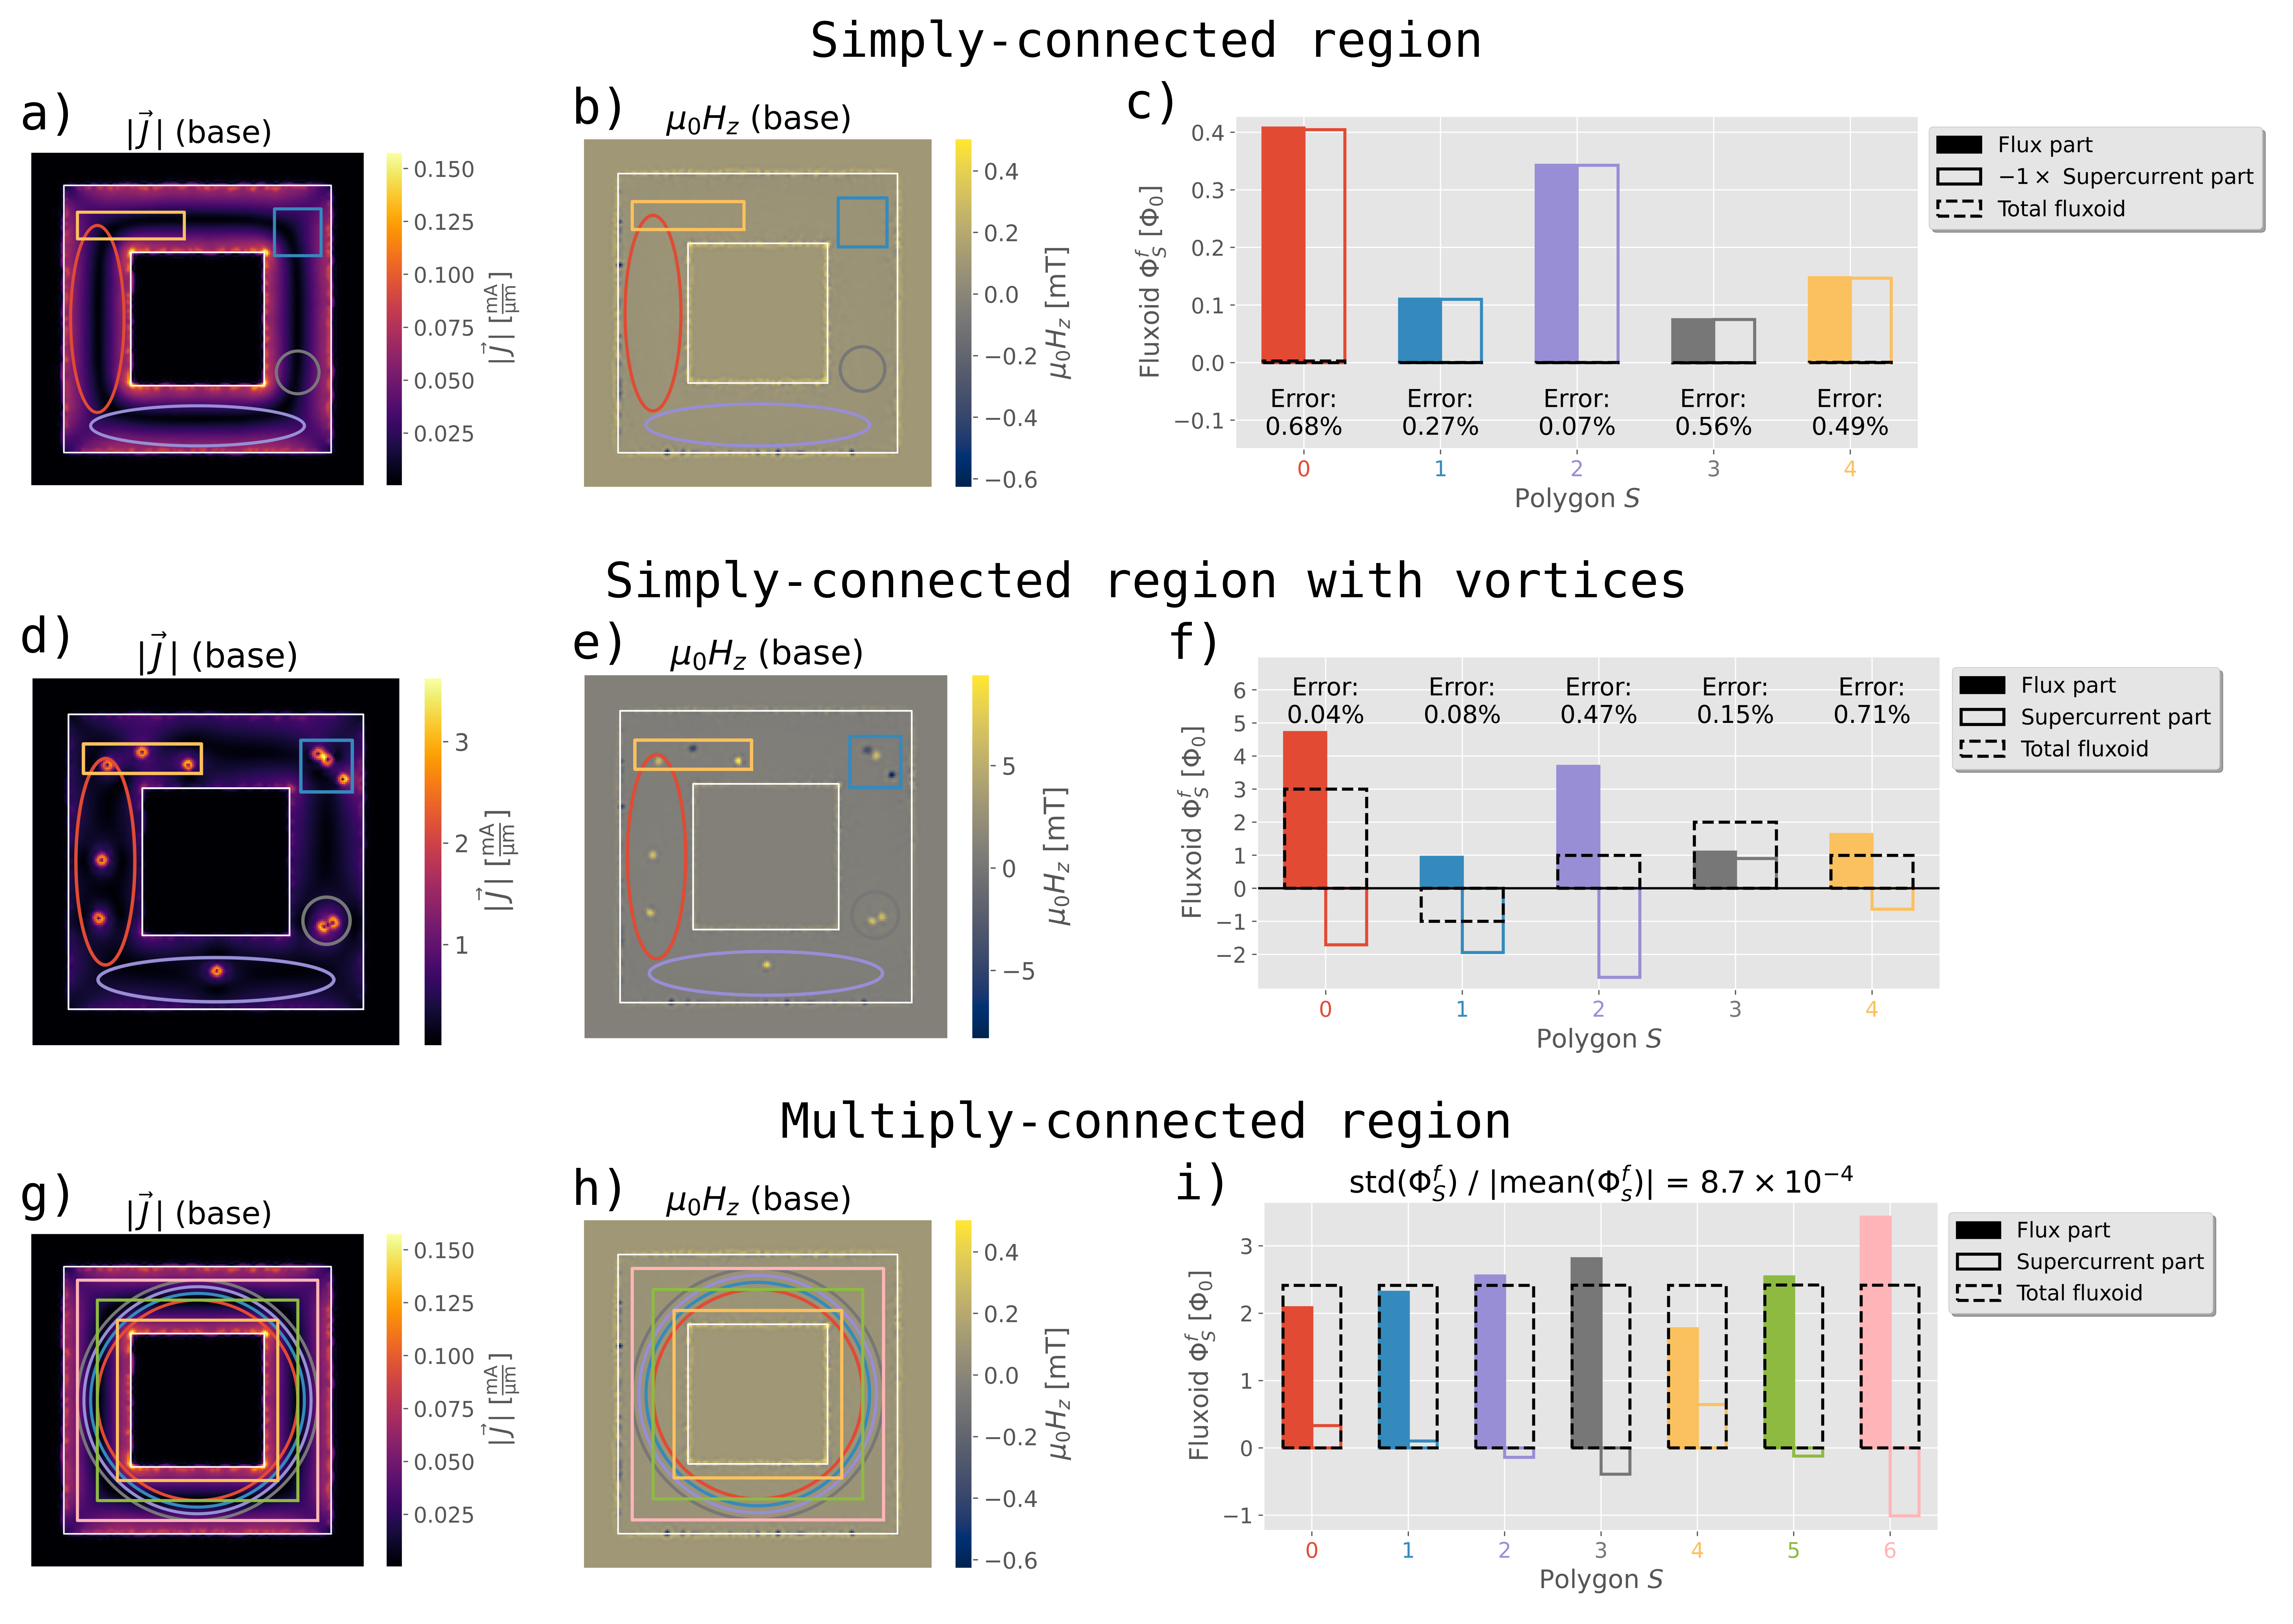
\includegraphics[width=\textwidth]{examples/images/fluxoid_combined.png}
%     \caption{Demonstration of the fluxoid properties listed in Section~\ref{section:examples:fluxoid} for a square ring with $\Lambda=1\,\mu\mathrm{m}$, inner side length $5\,\mu\mathrm{m}$, and outer side length $10\,\mu\mathrm{m}$, whose outline is shown with white lines in the left and middle columns, subject to a uniform applied field of 0.1 mT. The left and middle columns show the computed current density and out-of-plane-field, overlaid with several regions $S$ for which the fluxoids $\Phi^f_S$ are calculated using \inline{Solution.polygon_fluxoid()}. The corresponding fluxoids are shown in the right column. The colors of the paths in the left and middle columns correspond to the colors of the bars in the right column. Top row (a - c): The fluxoid $\Phi^f_S$ vanishes for all simply-connected regions containing no vortices. The errors in (c) are given by $|\Phi^f_S / \Phi^f_{S,\,\text{(flux part)}}|$. Middle row (d - f): For simply-connected regions containing a set of vortices $v$, each carrying flux $\Phi_v$, the fluxoid is given by $\sum_v\Phi_v$. In this case, the body of the square ring contains both ``positive'' ($\Phi_v=\Phi_0$, counter-clockwise circulating current) and ``negative'' ($\Phi_v=-\Phi_0$, clockwise circulating current) vortices, which appear in (e) as yellow and blue dots respectively. The expected value for the fluxoid for each region $S$ given in units of $\Phi_0$ by (number of yellow vortices lying inside $S$) - (number of blue vortices lying inside $S$), and the errors in (f) are reported relative to this expected value. Bottom row (g - i): Fluxoid path independence for the $n=0$ fluxoid state, shown here for both circular ($S = 0, 1, 2$) and square ($S=3, 4, 5$) paths. Here again, the errors are given by $|\Phi^f_S / \Phi^f_{S,\,\text{(flux part)}}|$.}
%     \label{fig:fluxoid}
% \end{figure}

\section{Numerical considerations}
\label{appendix:numerics}
While the numerical method described in Section~\ref{section:implementation} is generally quite robust, it can break down for certain extreme geometries. The stream function $g(x, y)$ represents the local magnetization or density of infinitesimal current loops. The $z$-component of the magnetic field at position $\vec{r}=(x, y, z)$ from a film $F$ with stream function $g$ lying in a plane parallel to the $x-y$ plane at vertical position $z'$ is given by (see Equations~\ref{eq:field_from_kernel} and \ref{eq:kernels}):
\begin{align}
\label{eq:hz-from-kernel}
\begin{split}
    H_z(\vec{r}) &= \int_F Q_z(\vec{r},\vec{r}')g(x', y')\,\mathrm{d}^2r',\,\text{where}\\
    Q_z(\vec{r}, \vec{r}') &=  \frac{2(z-z')^2-\rho^2}
            {4\pi[(z-z')^2+\rho^2]^{5/2}}
\end{split}
\end{align}
and $\rho=\sqrt{(x-x')^2+(y-y')^2}$. Eq.~\ref{eq:hz-from-kernel} is exact for a continuous stream function $g$. However, the discretized version of Eq.~\ref{eq:hz-from-kernel}, in which the double integral over the film area $F$ is replaced by a sum over triangular mesh elements, is only valid if $z-z'$, the vertical distance between the film and the point at which the field is being evaluated, is larger than the typical distance $\delta r$ between vertices in the mesh representing the film. For $z-z'\lesssim\delta r$, the field $H_z(\vec{r})$ resembles that of a set of isolated dipoles located at the mesh vertex positions, rather than that of a continuous sheet of current. This can lead to unphysical results when evaluating the field very close to the surface of a film (for example using \inline{Solution.field_at_position()}), or when solving models involving multi-layer structures where the vertical spacing between layers is much smaller than the lateral extent of the films, in which case the iterative calculation (Section~\ref{section:model:multilayer}) may not converge.

The latter case---mutli-layer structures with closely-spaced layers---is the most challenging class of problem to solve because the iterative method used to solve multi-layer structures (Section~\ref{section:model:multilayer}) is memory-intensive for models with a large mesh (many vertices $v$ and triangles $t$) and/or many layers $L$. As mentioned in Section~\ref{section:model:multilayer}, at each iteration of this process, we update the applied field $H_{z,\,\mathrm{applied}}(\vec{r}, z_\ell)$ at each layer $\ell$ based on the currents flowing in all other layers $m\neq\ell$, according to

\begin{equation}
    H_{z,\,\mathrm{applied}}(\vec{r}, z_\ell) \to
    H_{z,\,\mathrm{applied}}(\vec{r}, z_\ell)
    + \sum_{m\neq\ell}
    \int_{S_m} Q_z(\vec{r},\vec{r}')g_m(\vec{r}')\,\mathrm{d}^2r',
    \label{eq:iterative}
\end{equation}
where $S_m$ is surface of all films in layer $m$ and $g_m$ is the stream function for layer $m$. For a model with $L$ layers, at each iteration Eq.~\ref{eq:iterative} requires the calculation of $\binom{L}{2} = L(L-1)/2$ kernel matrices $\mathbf{Q_z}$, each of which is a dense $v\times t$ floating point matrix. Typically the number of mesh vertices is approximately half the number of triangles ($v\approx t / 2$), so for a mesh with $t=10,000$ triangles, each of these $\mathbf{Q_z}$ matrices is roughly 400 MB (200 MB) if using 64-bit double-precision floats (32-bit single-precision floats). Furthermore, each iteration requires performing $2\binom{L}{2} = L(L-1)$ sums involving $\mathbf{Q_z}\cdot\mathbf{g}_m$, where $\mathbf{g}_m$ is the $n\times1$ vector defining the stream function in layer $m$ evaluated at the center of each triangle in the mesh.

% To avoid redundant computation at each iteration and running out of memory during the iterative process, the $\mathbf{Q_z}$ matrices are computed once during the first iteration, cached to a temporary directory on disk, and loaded from disk during subsequent iterations, such that only a single $\mathbf{Q_z}$ is in memory at any given time. If running \SuperScreen on a machine with both hard disk (HDD) and solid state disk (SSD) storage, one should ensure that Python uses a temporary directory located on a solid state disk to avoid a significant performance penalty due to hard disk read/write speeds. See the documentation for the \inline{tempfile} module of the Python standard library for more details. Both the amount of computation needed per iteration and the number of iterations required to reach a certain level of convergence (quantified, for example, by the fractional change in flux through each polygon in the model from one iteration to the next)

\section{Parallel processing}
\label{section:parallel}
As discussed above, one can solve many models involving the same \inline{Device} in parallel across multiple CPUs using the \inline{superscreen.solve_many()} function. The recommended method for parallel processing is using \inline{ray}, a library for distributed computing using shared memory~\cite{Moritz2018-mt}. Note that at the time of writing, \inline{ray} support for Windows is experimental and under active development. \SuperScreen also supports parallel processing using the \inline{multiprocessing} module from the Python standard library, however this is generally less efficient than \inline{ray} in this application.

There are three ways to invoke \inline{ray} from \SuperScreen when running on a single machine, e.g. a multi-core CPU. The first is to simply pass the keyword argument \inline{parallel_method="ray"} when calling \inline{solve_many()}. This will automatically create a \inline{ray} cluster using all available physical CPU cores, solve the models in parallel, and then shut down the cluster before returning. The second method is to manually create a \inline{ray} cluster using the \inline{ray} Python application programming interface (API) prior to calling \inline{solve_many(..., parallel_method="ray")}, as demonstrated in Code Block~\ref{code:ray-python}. The third method is to start a \inline{ray} cluster using the command line interface (CLI), then connect to the existing cluster using the Python API prior to calling \inline{solve_many(..., parallel_method="ray")}, as demonstrated in Code Block~\ref{code:ray-cli}. One of the latter two methods should be used for finer control over the \inline{ray} cluster (number of CPUs to utilize, etc.).

\begin{code}
\begin{minted}[fontsize=\small]{python}
# Assume that we have already created a Device and put all
# other inputs to superscreen.solve_many() into a dictionary
# called other_kwargs.

import psutil
import ray

# Specify the number of CPUs/cores to allocate.
num_cpus = 3
# Use at most N processes for a machine with N physical CPUs.
num_cpus = min(num_cpus, psutil.cpu_count(logical=False))

# Start a ray cluster
ray.init(num_cpus=num_cpus)
# Solve the models
solutions, paths = superscreen.solve_many(
    parallel_method="ray",
    **other_kwargs,
)
# Shutdown the ray cluster
ray.shutdown()
\end{minted}
\end{code}

\begin{minipage}{\textwidth}
\begin{code}
\captionof{listing}{Starting and stopping \inline{ray} outside of \inline{superscreen.solve_many()} using the command line interface. See the \inline{ray} documentation for additional options in \inline{ray start}~\cite{ray-docs}.}
\label{code:ray-cli}
\begin{minted}[fontsize=\small]{bash}
# Start a ray cluster from the command line, e.g. bash
ray start --head --num-cpus=3
\end{minted}

\begin{minted}[fontsize=\small]{python}
# Assume that we have already created a Device and put all
# other inputs to superscreen.solve_many() into a dictionary
# called other_kwargs.
import ray
# Connect to the existing ray cluster.
# If more than one ray cluster is running, specify
# which to connect to using address="{ip}:{port}".
ray.init(address="auto")
# Solve the models.
solutions, paths = superscreen.solve_many(
    parallel_method="ray",
    **other_kwargs,
)
\end{minted}

\begin{minted}[fontsize=\small]{bash}
# Shut down the ray cluster from the command line
ray stop
\end{minted}
\captionof{listing}{Starting and stopping \inline{ray} outside of \inline{superscreen.solve_many()} using the Python API. See the ``API and Package Reference" section of the \inline{ray} documentation for additional options in \inline{ray.init()}~\cite{ray-docs}.}
\label{code:ray-python}
\end{code}
\end{minipage}

Running \inline{superscreen.solve_many()} in parallel across multiple nodes in a computing cluster is a simple extension to the method outlined in Code Block~\ref{code:ray-cli}, although the specifics depend upon the infrastructure of the cluster, e.g. job management software. See the ``Multi-Node Ray" section of the \inline{ray} documentation for more details~\cite{ray-docs}.
% Some applications of \SuperScreen may be ``embarrassingly parallel'' in the sense that all calls to \inline{superscreen.solve()} are completely independent. One such application is the scanning SQUID susceptometry simulation shown in Section~\ref{section:application}. In such cases, it may be simpler to avoid using \inline{ray} for shared memory and run many 

%% References
%%
%% Following citation commands can be used in the body text:
%% Usage of \cite is as follows:
%%   \cite{key}         ==>>  [#]
%%   \cite[chap. 2]{key} ==>> [#, chap. 2]
%%

%% References with bibTeX database:

\bibliographystyle{elsarticle-num}
\bibliography{references}

%% Authors are advised to submit their bibtex database files. They are
%% requested to list a bibtex style file in the manuscript if they do
%% not want to use elsarticle-num.bst.

%% References without bibTeX database:

% \begin{thebibliography}{00}

%% \bibitem must have the following form:
%%   \bibitem{key}...
%%

% \bibitem{}

% \end{thebibliography}


\end{document}

%%
%% End of file 